\documentclass[a4paper, 11pt]{article}

\usepackage[utf8]{inputenc}
\usepackage{verbatim}
\usepackage{moreverb}
\usepackage[english]{babel}
\usepackage[T1]{fontenc}
\usepackage{lmodern}
\usepackage{graphicx}
\usepackage{fancyhdr}
\usepackage{listings} 
\usepackage{lastpage}
\usepackage[top=3cm, bottom=3cm, left=2cm, right=2cm]{geometry}
\usepackage{color}
\usepackage{xcolor}

%font change
\renewcommand{\familydefault}{\sfdefault}

\newcommand{\HRule}{\rule{\linewidth}{0.5mm}}
\newcommand{\nl}{\\[0.1cm]}
\newcommand{\s}{\vspace{0.3cm}}
\newcommand{\smore}{\vspace{0.6cm}}

\usepackage{caption}
\DeclareCaptionFont{white}{\color{white}}
\DeclareCaptionFormat{listing}{\colorbox{gray}{\parbox{\textwidth}{#1#2#3}}}
\captionsetup[lstlisting]{format=listing,labelfont=white,textfont=white}

\lstset{frame=single}

\lstdefinelanguage{popc}{%
   morekeywords={%
   %od
      od, url, power, @, 100, 80, machine, POPString, search
  },
  sensitive=true,
  morestring=[b]',
}

\addto\captionsenglish{%
  \renewcommand{\listfigurename}{}%
	\renewcommand\refname{}
}



%Header and footer 
\pagestyle{fancy}
\fancyhead{}
\fancyfoot{}

%Header definition
\renewcommand{\headrulewidth}{0.5pt}
\lhead{ViSaG : Virtual Safe GRID}
\rhead{Version 1.5}

%Footer definition
\renewcommand{\footrulewidth}{0.5pt}
\cfoot{\today}
\lfoot{Valentin Clément}
\rfoot{Page \thepage ~on \pageref{LastPage}}

%remove indent for paragraph
\parindent0ex 

%\setlength{\parskip2ex}








%\pagebreak



\begin{document}

% TITLE INFORMATION

\begin{titlepage}
 
\begin{center}

\includegraphics[scale=0.3]{logo_eif.png}\\[1.5cm]
\textsc{\LARGE ViSaG - Virtual Safe GRID}\\[1.5cm]


\includegraphics[scale=0.3]{pic/logo_pop.png}\\[2cm]


\HRule \\[1cm]
{ \huge \bfseries POP-C++ Virtual-Secure (VS)}\\[0.5cm]
\textsc{\LARGE POP-C++ User and Installation manual : add-on}\\[1cm]
 
\HRule \\[5cm]
 
% Author and supervisor
\begin{minipage}{0.4\textwidth}
\begin{flushleft} \large
\textbf{Author:}\\
Valentin Clément
\end{flushleft}
\end{minipage}
\begin{minipage}{0.4\textwidth}
\begin{flushright} \large
\textbf{Date:} \today \\

\textbf{Revision:} 1.0
\end{flushright}
\end{minipage}
 
\vfill
  
\end{center}
 
\end{titlepage}

%\newpage \thispagestyle{empty} \mbox{}\newpage



\tableofcontents
\pagebreak
\section{Introduction}
Virtual - POP-C++ is a version of the POP-C++ middle-ware that would be able to run parallel objects into virtual machines. The development of this version is the core of the ViSaG project. A prototype version of Virtual - POP-C++ has been developed during a bachelor thesis project in the summer 2010. This version is called VirtualPOPC-1\cite{vpopc1}.\s

\textit{NOTE : } VirtualPOPC-1 will be referred as VPOP1 in the rest of this document.\s

This document is structured as follows:
\begin{itemize}
\item The next chapter is focusing on the weaknesses of the prototype developed during a Bachelor Thesis. 
\item The Chapter \ref{sec:repartition} aims to dispatch the work between the partner institutions working on this project. 
\item The Chapter \ref{sec:open_points} was written to helps the project team to take the right decisions concerning the future development on this project. 
\item Chapter \ref{sec:modif} explains all the modifications done on the first prototype to make the final version of POP-C++ for ViSaG.
\item Chapter \ref{sec:gen_mod} just explains small modifications that are general to all POP-C++ versions.
\item Chapter \ref{sec:security} tells what we think about the security of our new version.
\item Chapter \ref{sec:test} focuses on functional and performance tests. 
\item Chapter \ref{sec:future} gives some ideas for future development. 

\end{itemize}

Keep in mind this document has been updated during the whole development process. The firsts chapters have been written before the actual development of the new versions. 




\section{Requirements for Virtual POP-C++}
\label{weakness}
This chapter aims to identify the weaknesses and the missing elements of VPOP1. At the end of this chapter, all the modifications that have to be brought for the final version to be produced for the ViSaG project will be summarized and shared between the EIA-FR and the HEPIA.\s


\subsection{Hypervisor related data}
In VPOP1, all the data related to the hypervisor connection are saved as environment variables. These data should be saved in the JobMgr config file located at \textit{POPC\_LOCATION}/etc/jobmgr.conf. The hypervisor password should be encrypted and not saved in clear.\s

\textbf{Files to be modified :} ./lib/jobmgr.cc, ./include/jobmgr.ph, ./script/popc\_setup.in\s

\textbf{Work done:}\\
All the hypervisor related data are now stored in a file located in the POP\_LOCATION/etc/virtual.conf. These data could evolve with the changes that will be done in the future. \s

\textbf{Decision:}\\
The whole configuration file will be encrypted with a symmetric algorithm. More information about this point are given later in this document. 

\subsection{Code injection in wrapper}
In the wrapper used to contact the hypervisor, some methods execute a shell command. As the command executed is prepared in the method, some malicious codes could be injected. To avoid this code injection, the commands should be controlled before their execution.\s

\textbf{Files to be modified : } ./lib/ESXWrapper.cc\s

\textbf{Work done:}\\
The wrapper does not use external command any more. \s

\textbf{Decision:}\\
The methods using shell command will be replaced by VIX API code. The cloning process will run some external command but this process is not executed in the wrapper. We are currently looking to implement the cloning function inside libvirt itself. 

\subsection{POP Application Identifier}
A POP Application Identifier must be created for any POP-C++ application. This ID must be sent with the resource discovery request. A virtual node will create only one virtual machine (VM) per application. Any parallel object of the same application running on the same virtual node will be executed in the same VM. This VM will be shutdown at the end of the application or after a specified idle time.\s

\textbf{File to be modified : } ./lib/request.cc, ./include/request.h, ./lib/jobmgr.cc, ./lib/appservice.ph, ./lib/ap- pservice.cc, ./lib/popc\_search\_node.cc\s

\textbf{Work done:}\\
The POPAppId is passed in the resource discovery process and the admin-VM takes it into consideration for the workers management. The VM is shutdown when it has no more jobs running on it. This step is finished.\s

\textbf{Decision:}\\
The VM could be shutdown when the application is finished. A message must be send to all nodes to shutdown the VM associated with the application. This decision has been implemented in POP-C++. More information about this implementation can be found later in this document. 

\subsection{Installation of admin and worker VM}
The installation of the environment on the admin and worker VM could be the source of many problems. This installation should be as automatic as possible (missing library, ssh key generation, ssh\_config, cloning VM ...).\s

\textbf{Files to be modified : } ./script/popc\_setup.in, ./configure.ac\s

\textbf{Work done:}\\
The configure script is no able to accept the option "--enable-virtual". This option allows the user to compile POP-C++ in the Virtual version. Without this option, the standard version is compiled. To be able to compile two different versions, a VirtualJobMgr and a VirtualPOPCSearchNode have been implemented. All the virtual version is implemented by overwriting basic function of the standard JobMgr and POPCSearchNode. This step is almost done. There is some work to do in the installation script (remove useless questions, check SSH, generate key if not present ...). \s

\textbf{Decision:}\\
The popc\_setup script as soon as we have the time. 

\subsection{Cloning VM}
The worker VM must be cloned as much as needed on a virtual node. This process should be done before needing the VM. As the cloning process takes some time, it could be a good idea to start the cloning process when just one VM is available. 

For example, a node running Virtual POP-C++ is using 3 workers. When the second worker is reserved (just one more worker free), the cloning process starts to make a new worker. The maximum number of worker on a node must be defined during the installation.\s

\textbf{Files to be modified: } Not defined \s

\textbf{Work done:}\\
Some experiments with VIX and with a home made script. Nothing implemented in POP-C++ for the moment. HEPIA has maybe some hints to give about this process. \s

\textbf{Decision:}\\
Using the hard copy solution from a C++ code. Asking HEPIA if they could find a better solution. The cloning process starts when there are only X free VM left. The number of VM prepared in advance is specified as an option.

\subsection{Preparation of the worker VM}
In the current version, the preparation of the VM is not very reliable. In fact, during this preparation, the ESXWrapper will try to get the VM IP. After three attempts, the preparation will fail if the IP is not discovered. This process should be optimized and maybe done differently.\s

\textbf{Files to be modified : } ./lib/ESXWrapper.cc\s

\textbf{Work done:}\\
Solved the waiting problem. Try with the VIX API, which seems to be more reliable than the command line tool. Nothing is implemented with the VIX API in POP-C++ for the moment but I got a test program sample. \s

\textbf{Decision}\\
Using the VIX API to retrieve the IP address. DHCP renewal must be done before retrieving the address (this point is open because more information on DHCP must be found).

\subsection{JobMgr - Management of VM and jobs}
As the JobMgr running on the admin-VM must be able to manage several worker-VM, this JobMgr must be modified to include the management of different VM with the POPAppID. This management must include the startup, check during runtime and shutdown of a VM for an application.\s

\textbf{Files to be modified : } ./lib/jobmgr.cc, ./lib/ESXWrapper.cc\s

\textbf{Work done:}\\
Modify the check and reserve process for taking into consideration the management of several workers. Ability to run several objects of the same application on the same VM. Host resource management must be defined. \s

\textbf{Decision:}\\
The admin-VM manage all the resource on the node. The all node is seen as one POP-C++ node. The VMs are just a way to encapsulate the parallel objects execution.

\subsection{WorkerDeamon}
The WorkerDeamon is in charge of the key exchange between the admin-VM and the worker-VM. This worker is not well developed. Here are some hints to find a different way to exchange the keys:\s

\textbf{Hints:} 
\begin{itemize}
\item The keys could be passed during the installation of the environment. Once one worker-VM is cloned, its virtual disk could be mounted on the admin-VM and the admin-VM key could be write in the file system.
\item The keys could be passed during the installation of the environment. Once one worker-VM is cloned, it could be started and the keys exchanged before taking a snapshot of it. 
\item A POP-C++ parallel object could be used to do that. The creation of a virtual POP-C++ service as a parallel object could run independently on the worker-VM. This parallel object could be contacted by the admin-VM and the keys could be exchanged.
\end{itemize}

\textbf{Work done:}\\
Test program with the VIX API and the copy file function. This solution seems to work perfectly. With this solution, the POP-C++ Security Manager running on the admin-VM could manage the keys of all workers. Nothing has to run on the worker. \s

\textbf{Decision:}\\
Use the VIX API to do this task. Ask HEPIA is they could find another way to communicate between the admin-VM and the worker-VM. We are aware that this solution is less generic.\\
Some other solution must be explored such as shared disk or shared network (libvirt).

\subsection{Pseudo-Main}
As we want to run a POP-C++ application in a full secured environment, the main of the application should be launched in a VM too. To do that, a pseudo-main could redirect the real main on a VM and launch it in a secure way.\s

\textbf{Files to be modified} : POP-C++ compiler (paroc\_main)\s

\textbf{Work done:}\\
Nothing for the moment.\s

\textbf{Decision:}\\
This point is open. We can offer an option to let the user choose to run the main in a VM or not.

\subsection{Fusion of POP-C++ 1.3.1 beta JS1.2 and Virtual-POP-C++}
The Virtual version of POP-C++ must be merged with the secure version of the POP-C++. This will make the ViSaG version of POP-C++.\s

\textbf{Work done:}\\
Prepare the configure script to be able to accept the option "--enable-secure". 

\subsection{Minimal Linux distribution}
The admin-VM should be as light as possible. In fact, this admin-VM will never run a parallel object for a POP-C++ application. This VM is only in charge of the management of the others VM known as worker-VM. Due to this fact, this VM should run the lightest distribution of Linux that can run the POP-C++ Global Services. This distribution should also support "libvirt" and the "vSphere CLI" libraries.\s

\textbf{Work done:}\\
Nothing for the moment. HEPIA could work in this. 

\subsection{Add restrictions on SSH}
It's possible to add restrictions on the use of SSH for a specific public key. It could be a good idea to allow only what we really need for POP-C++ (SSH tunnelling and the popcrun command). This restriction are added with the public key in the "authorized\_keys" file. The POP-C++ Security Manager should be able to add these restrictions when it writes a new key. \s

We can imagine that all SSH restrictions are defined during the installation of POP-C++. These information will be passed to the PSM for future usage.\s

\textbf{Work done:}\\
Nothing for the moment.\s

\textbf{Decision:}\\
Add SSH restrictions. Only enable the tunnelling and the use of the "popcobjrun" command.

\subsection{ESXi user and restriction}
VMware ESXi has a user and group management system. It would be more secure to create a specific user for Virtual POP-C++ and allow only the specific action related to its usage. \s

The administrator of the ESXi platform has many privileges that can be granted or revoked. All the actions about users and groups must be done from the vSphere Client. \s

\textbf{Work done:}\\
Nothing for the moment.\s

\textbf{Decision}\\
Using the root account for the moment. When the full version of POP-C++ Virtual and Secure will be ready, ask HEPIA to do some test if we can reduce the rights and use a different account.

\subsection{Testing}
A full protocol of test must be done on the full version of POP-C++ for ViSaG. The tests must contain : 
\begin{enumerate}
\item Stress test to check the concurrency problems.
\item Performance test to be able to measure the overhead and make some optimizations. 
\item Memory test using mudflap or valgrind to check any memory leaks. 
\end{enumerate}

\subsection{Encrypted file system}
The possibility to use an encrypted file system on the VM could enforce the security of the whole project. This point is open and must be studied. 

\pagebreak
\section{Repartition}
\label{sec:repartition}
This section suggests a repartition of the work between the EIA-FR and the HEPIA (the two schools working on the ViSaG project and more specifically on the lower level of this project).\s

Theoretical, the EIA-FR is in charge of the major modifications of the POP-C++ middle-ware and the HEPIA is in charge of the global VM management. The task above will be 


\begin{center}
\begin{tabular}{|p{1.5cm}|p{7.5cm}|p{2cm}|p{4cm}|}
\hline
\textbf{Section} & \textbf{What ?}	& \textbf{Who ?} & \textbf{Priority} \\ \hline
2.1 & Hypervisor informations & EIA-FR & Medium (Done, except password crypt) \\ \hline

2.2 & Code injections in wrapper & EIA-FR & Medium \\ \hline

2.3 & POP Application Identifier & EIA-FR & (DONE!)\\ \hline

2.4 & Installation of admin and worker VM & EIA-FR & (DONE!) \\ \hline

2.5 & Cloning VM & HEPIA (EIA-FR) & On the way \\ \hline

2.6 & Preparation of worker VM & EIA-FR & (Will be done with VIX) \\ \hline

2.7 & JobMgr - management & EIA-FR & (on the way) \\ \hline

2.8 & WorkerDeamon & EIA-FR & High (VIX API)\\ \hline

2.9 & PseudoMain & EIA-FR & Medium \\ \hline

2.10 & Fusion & EIA-FR & High\\ \hline

2.11 & Minimal Linux distribution & HEPIA & Medium \\ \hline

2.12 & Add restrictions to SSH & EIA-FR & High \\ \hline

2.13 & ESXi user and restrictions & HEPIA & Medium \\ \hline

2.14 & Testing & HEPIA and EIA-FR & High (wait full version) \\ \hline

2.15 & Encrypted file system & HEPIA and EIA-FR & Medium \\ \hline

\end{tabular}
\end{center}\s


\pagebreak
\section{Open points and information}
\label{hints}

This chapter regroups some points that are still open and some useful information for taking decisions about the future step to do in the ViSaG project. Some of those points have been discussed and a decision has been made (see Chapter \ref{weakness} for the decisions made). 

\subsection{VMware VIX API}
VMware provides a C based API to interact with VM. This API has some interesting function that could help us in the development of the Virtual version of POP-C++. These functions are: 

\begin{itemize}
\item \textbf{VixVM\_Clone} : cloning an existent VM with snapshot (unimplemented with ESXi).
\item \textbf{VixVM\_CopyFileFromGuestToHost} : copy a file from the guest VM (worker) to the host VM (admin)
\item \textbf{VixVM\_CopyFileFromHostToGuest} : copy a file from the host VM (admin) to the guest VM (worker)
\item \textbf{VixVM\_ReadVariable} : some property of the VM (ip address) could be read like that.
\end{itemize}

The VIX 1.10 API reference can be found at following URL: \\
http://www.vmware.com/support/developer/vix-api/vix110\_reference/\s

\textit{NOTE:} The "product support" section of the reference cited above mentions that the function VixVM\_Clone is only supported on VMware Workstation platform.\s

\textit{REMARK:} Using a proprietary API could be a little bit restrictive but it would also be much more reliable than the use of command line tools that are also proprietary.

\subsection{Cloning}
The cloning process of a VM is going like this : 

\begin{enumerate}
\item Create a new folder on the data store (vifs --mkdir).
\item Copy every files from the original VM folder to the new folder (except log files) (vmkfstools -i).
\item Modify the "display name" of the VM (vifs -g, awk, vifs -p).
\item Register the new VM in the inventory (vmware-cmd).
\item Start the VM (vmware-cmd).
\end{enumerate}

This solution could be easily implemented in the current version of Virtual POP-C++ (a shell script is already working for that purpose). \s

\textit{NOTE(1):} None of the VIX API or LIBVIRT is able to provide this function for the moment. \s

\textit{NOTE(2):} When a worker is cloned, the SSH pairs is the same on the original VM and on the cloned VM. This is not a problem for the functionality of POP-C++. It could be a bad practice from a security point of view. We could force the worker to generate new key after the cloning process by launching a command with VIX.  

\subsection{Key exchange with the VM}
The workerDeamon must be changed because now it is not reliable and not secure enough. In addition, with the secure version, the worker VM must be able to do more than just receive a key.  Here are the needs for the key exchange:

\begin{itemize}
\item The admin must be able to read the PKI of the worker.
\item The worker must accept PKI from the admin.
\end{itemize}

The VIX API gives a way to copy a file from a host to a guest. This API also gives a way to execute a program on the guest.\s

\subsection{Names and addresses used in Virtual POP-C++}
POP-C++ and its virtual version use different mechanism to retrieve a machine identity. Here is a brief summary of methods used in the virtual version of POP-C++ currently in development.\s


\textbf{Between Global Services}\\
Between the global services, either the IP address or the hostname could be used. \s

\textbf{Between VM-admin and VM-worker}\\
Between the VM-admin and the VM-worker two different kind of identification are used. Firstly, when the admin reverts the worker to the correct snapshot, the "display name" of the VM is used. This "display name" is a notion from VMware ESXi. A VM is registered under this name in the vSphere inventory (see Figure \ref{fig:vsphere}). With this "display name", the admin is able to retrieve the IP address of the worker. Once the admin knows the worker IP address it can communicate directly with the worker (at this point the hostname could also be used). 

\begin{figure}[ht]
	\caption{vSphere Client - inventory (display name)}
  	\centering
	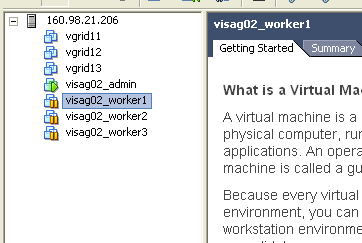
\includegraphics[scale=1.0]{../inventory.png}
	\label{fig:vsphere}
\end{figure}

\subsection{DHCP}
Using the DHCP service for the worker is not without any risks. This section will list the known issues about its usage. \s

\textbf{Lease on a suspended VM}\\
DHCP service uses lease for IP address. When a VM is reverted to a snapshot from a "shutdown state" or a "suspended state", the lease could be expired and the IP address may change after a few minutes. This behaviour could make the POP-C++ application crash. A solution to this problem is to force the VM to ask for a new lease when it is reverted. In this case the IP address would be changed before any execution on the worker and the application could run normally. 







\pagebreak
\section{Modifications related to ViSaG}
\label{sec:modif}
\label{modifications}

This chapter is a review of the modifications made on the prototype (VPOP1) to make a fully functional version of POP-C++ VS for the ViSaG project. The new version includes also the modifications made on POP-C++ for the Secure version (for more information, please refer to "POP-C++ over SSH Tunnel"\cite{popcssh}).

\subsection{Compilation of four different versions of POP-C++}
As POP-C++ could be installed for different usage (cluster, secure, virtual ...), the ability to compile the right version is fundamental. There are four different ways to compile POP-C++ by passing option to the configure script. Here are the four versions : 

\begin{itemize}
\item \textbf{POP-C++} Standard version (cluster, local test...) : configure without options
\item \textbf{POP-C++ S}ecure version (with SSH tunnelling) : configure with the option --enable-secure
\item \textbf{POP-C++ V}irtual version (with worker virtualization - Admin Node only) : configure with the option --enable-virtual
\item \textbf{POP-C++ V}irtual-\textbf{S}ecure version (SSH tunnelling and worker virtualization - for Admin Node only) : configure with the options --enable-virtual --enable-secure
\end{itemize}

\textit{NOTE:} Be aware that all the versions are not fully compatible with each other. For the moment, standard and virtual version can be used together and secure and virtual secure versions can be used together. A compatibility table is available in the document "POP-C++ Virtual-Secure : POP-C++ User and Installation manual add-on"\cite{popc_vs_addon_manual}.\s

\begin{figure}[ht]
	\caption{POP-C++ Global Services}
  	\centering
	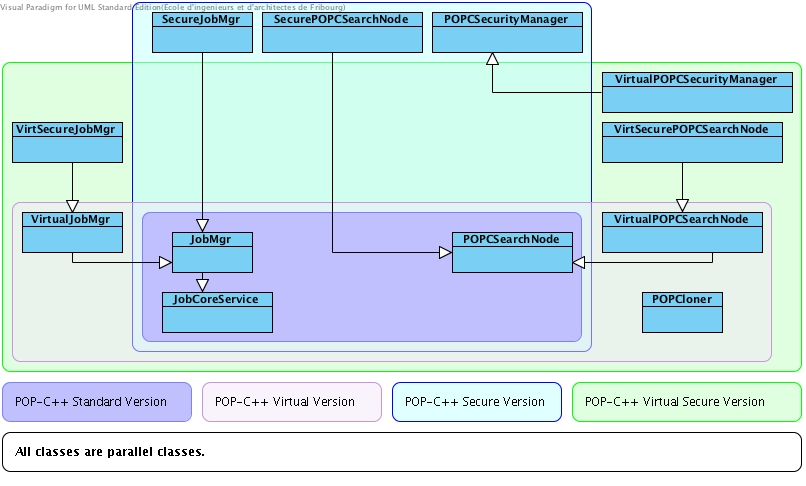
\includegraphics[width=1.0\textwidth]{./pic/global_service_cd.jpg}
	\label{fig:global_service_cd}
\end{figure}

To make this compilation possible, the POP-C++ Global Services has been specialized with new classes. Figure \ref{fig:global_service_cd} shows the new class diagram of the POP-C++ Global Services in each version.\s

All the modifications related to the VS version are now made in the VirtSecureJobMgr, VirtualJobMgr, VirtSecurePOPCSearchNode, VirtualPOPCSearchNode and VirtualPOPCSecurityManager. These modifications will let the future versions of POP-C++ evolve easily one relative to another.\s

To configuration script will create one of the four follwoing variables : STANDARDSUPPORT, VIRTSUPPORT, SECURESUPPORT, VIRTSECURESUPPORT. The created variable is used in the input makefile (Makefile.am) to define to right compilation process. \s

After any modification in the configure.ac file, it is very important to run the following command to generate the new configure script. 
\begin{lstlisting}
autoreconf
\end{lstlisting}\s

\textbf{Files created:} ./lib/virtual\_jobmgr.ph, ./lib/virtual\_jobmgr.cc, ./lib/virtual\_secure\_jobmgr.ph, ./lib/virtual\_secure\_jobmgr.cc, ./lib/virtual\_popc\_search\_node.ph, ./lib/virtual\_popc\_search\_node.cc, ./lib/virtual\_secure\_popc\_search\_node.ph, ./lib/virtual\_secure\_popc\_search\_node.cc, ./lib/virtual\_popc\_secu rity\_manager.ph, ./lib/virtual\_popc\_security\_manager.cc,
 ./services/secure\_jobmgr\_obj.cc,  ./services/virtual\_secure\_jobmgr\_obj.cc,  ./services/secure\_popc\_search\_node\_obj.cc,  ./services/virtual\_secure\_popc \_search\_node\_obj.cc,  ./services/virtual\_popc\_security\_manager\_obj.cc \s

\textbf{Files modified:} ./configure.ac, ./lib/jobmgr.ph, ./lib/jobmgr.cc, ./lib/popc\_search\_node.ph, ./lib/Makefile.am, ./lib/interface.cc, ./script/popc\_setup.in, ./services/Makefile.am\s



%
% HYPERVISOR INFORMATION
%
\pagebreak
\subsection{Hypervisor information}
Instead of being stored in environment variables, the information relative to the hypervisor connection have been stored in the Virtual JobMgr configuration file. This file is located under \textit{POPC\_LOCATION}/etc/virtu- al.conf. The installation script writes the information directly into this configuration file instead of writing them into a script that initialize the environment variables. \s

The VirtualJobMgr constructor retrieves all the information stored in the configuration file. These values are stored into attributes and used when needed.\s

\textbf{Files modified: } ./lib/virtual\_jobmgr.cc, ./lib/virtual\_jobmgr.ph, ./script/popc\_setup.in\s

\subsubsection{Hiding password in POP-C++ Virtual Configuration}
The configuration file used in the virtual version of POP-C++ contains some sensible data. These data must be encrypted to avoid unwanted usage of it. To do this task, we choose to encrypt the whole configuration file. This section explains the different algorithm available to this this job and the one we choose in POP-C++ VS.\s


\textbf{Encryption/Decryption algorithm}\\
There are two main category of encryption/decryption algorithm. These two categories are explained below:

\begin{itemize}
\item \textbf{Symmetric encryption}: using one key two encrypt and decrypt. Figure \ref{fig:symmetric_algo}A shows the encryption/decryption process of a symmetric algorithm.
\item \textbf{Asymmetric encryption}: using a pair of private/public keys. One key is used to encrypt the message and the second to decrypt it. Figure \ref{fig:asymmetric_algo}B shows the encryption/decryption process of an asymmetric algorithm. In this kind of encryption, we could even use an external dongle that manages the encryption and the decryption of the file. 
\end{itemize}
 
 \begin{figure}[ht]
	\caption{Symmetric and Asymmetric encryption algorithm}
  	\centering
	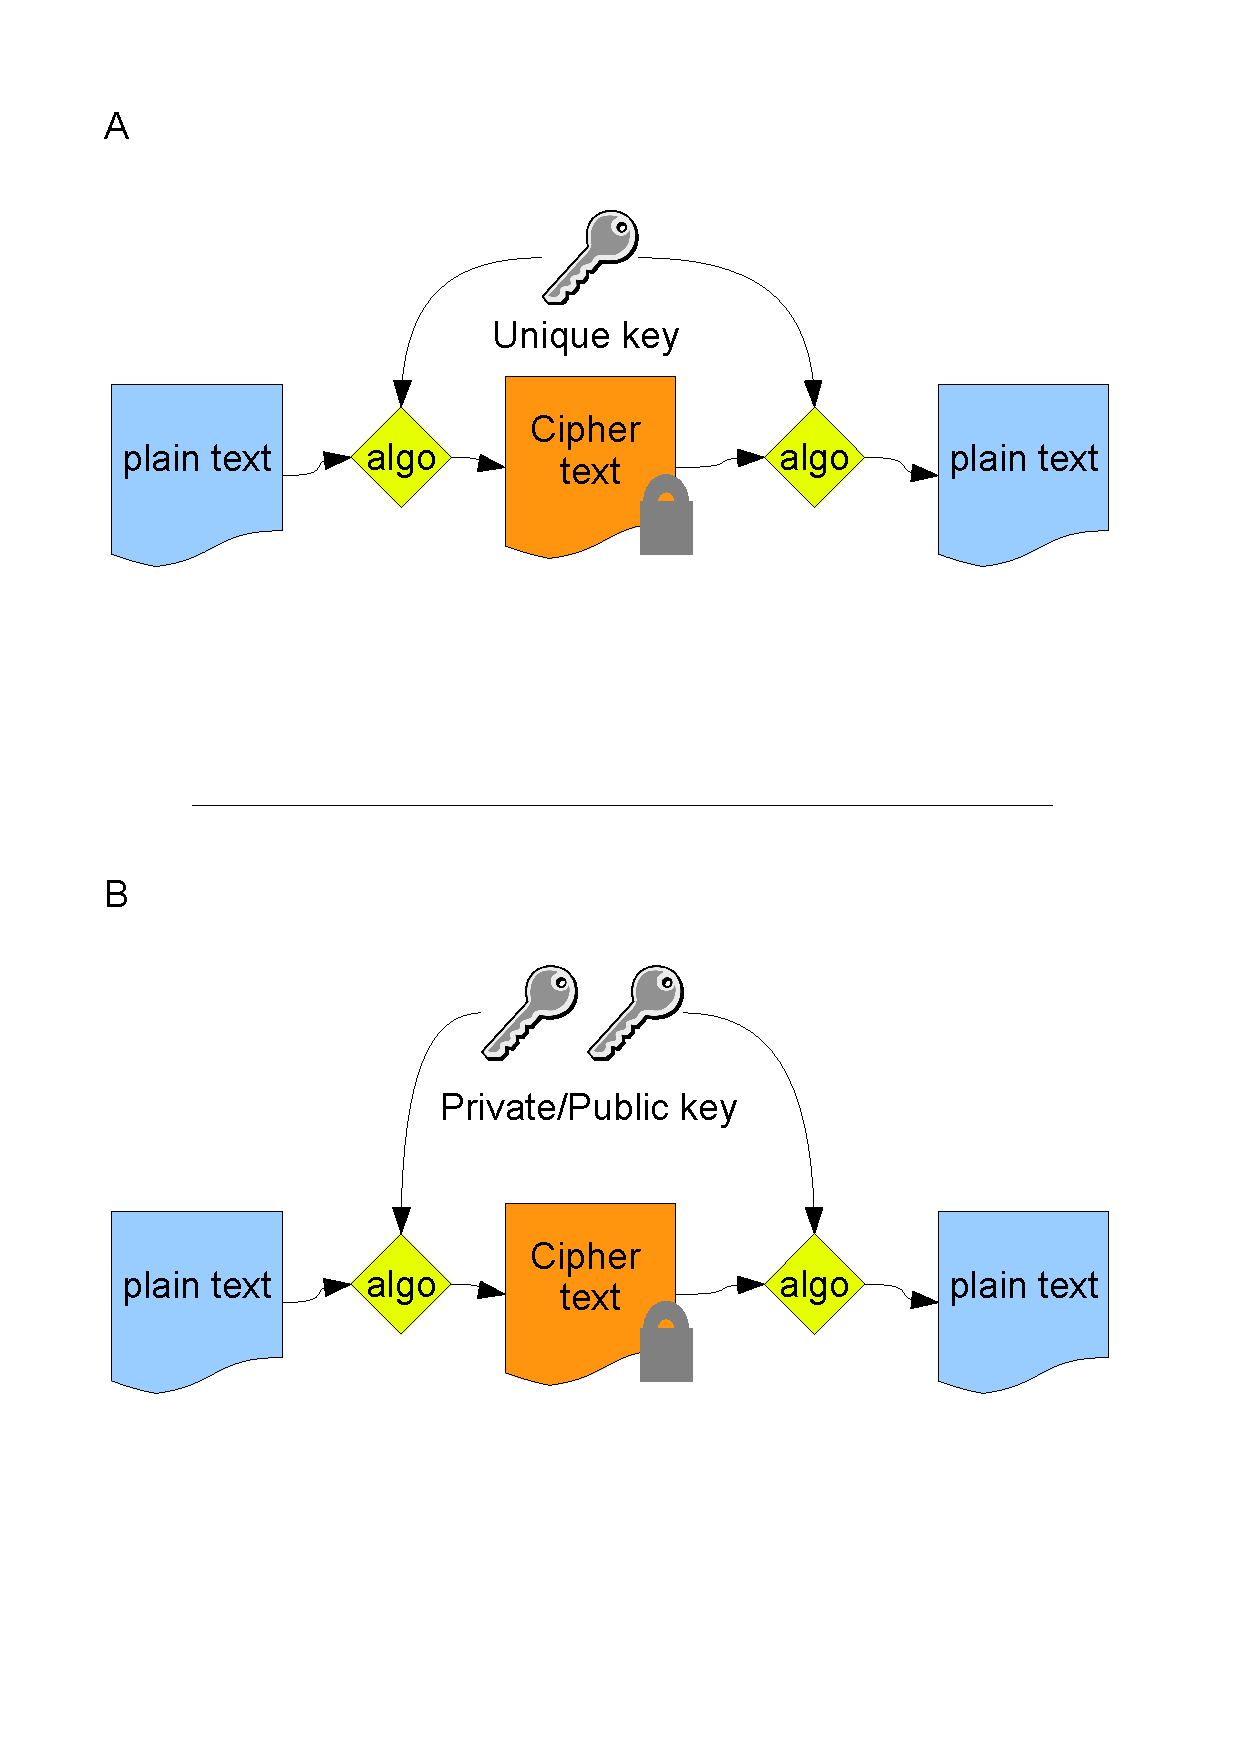
\includegraphics[width=0.7\textwidth]{./pic/encrypt_algo.pdf}
	\label{fig:asymmetric_algo}
\end{figure}

\pagebreak
\textbf{Algorithm used in POP-C++ VS}\\
To encrypt the configuration file used in the POP-C++ VS, we choose to use the AES (rijndael) algorithm. The first step is to generate a key and cipher the information about the virtual configuration. Figure \ref{fig:cipher1} shows this first step. During the compilation of POP-C++, a key is generated and integrated to the executable of POP-C++. A small program is compiled to be able to cipher the information about the virtual configuration during the installation of POP-C++. This program is called \textbf{popcipher}. As shown in Figure \ref{fig:cipher1}, the JobMgr configuration file is not encrypted at all. Only the virtual configuration file is processed by \textbf{popcipher} as this file includes some important passwords. 

\begin{figure}[ht]
	\caption{POP-C++ Virtual Configuration - Cipher - Step 1}
  	\centering
	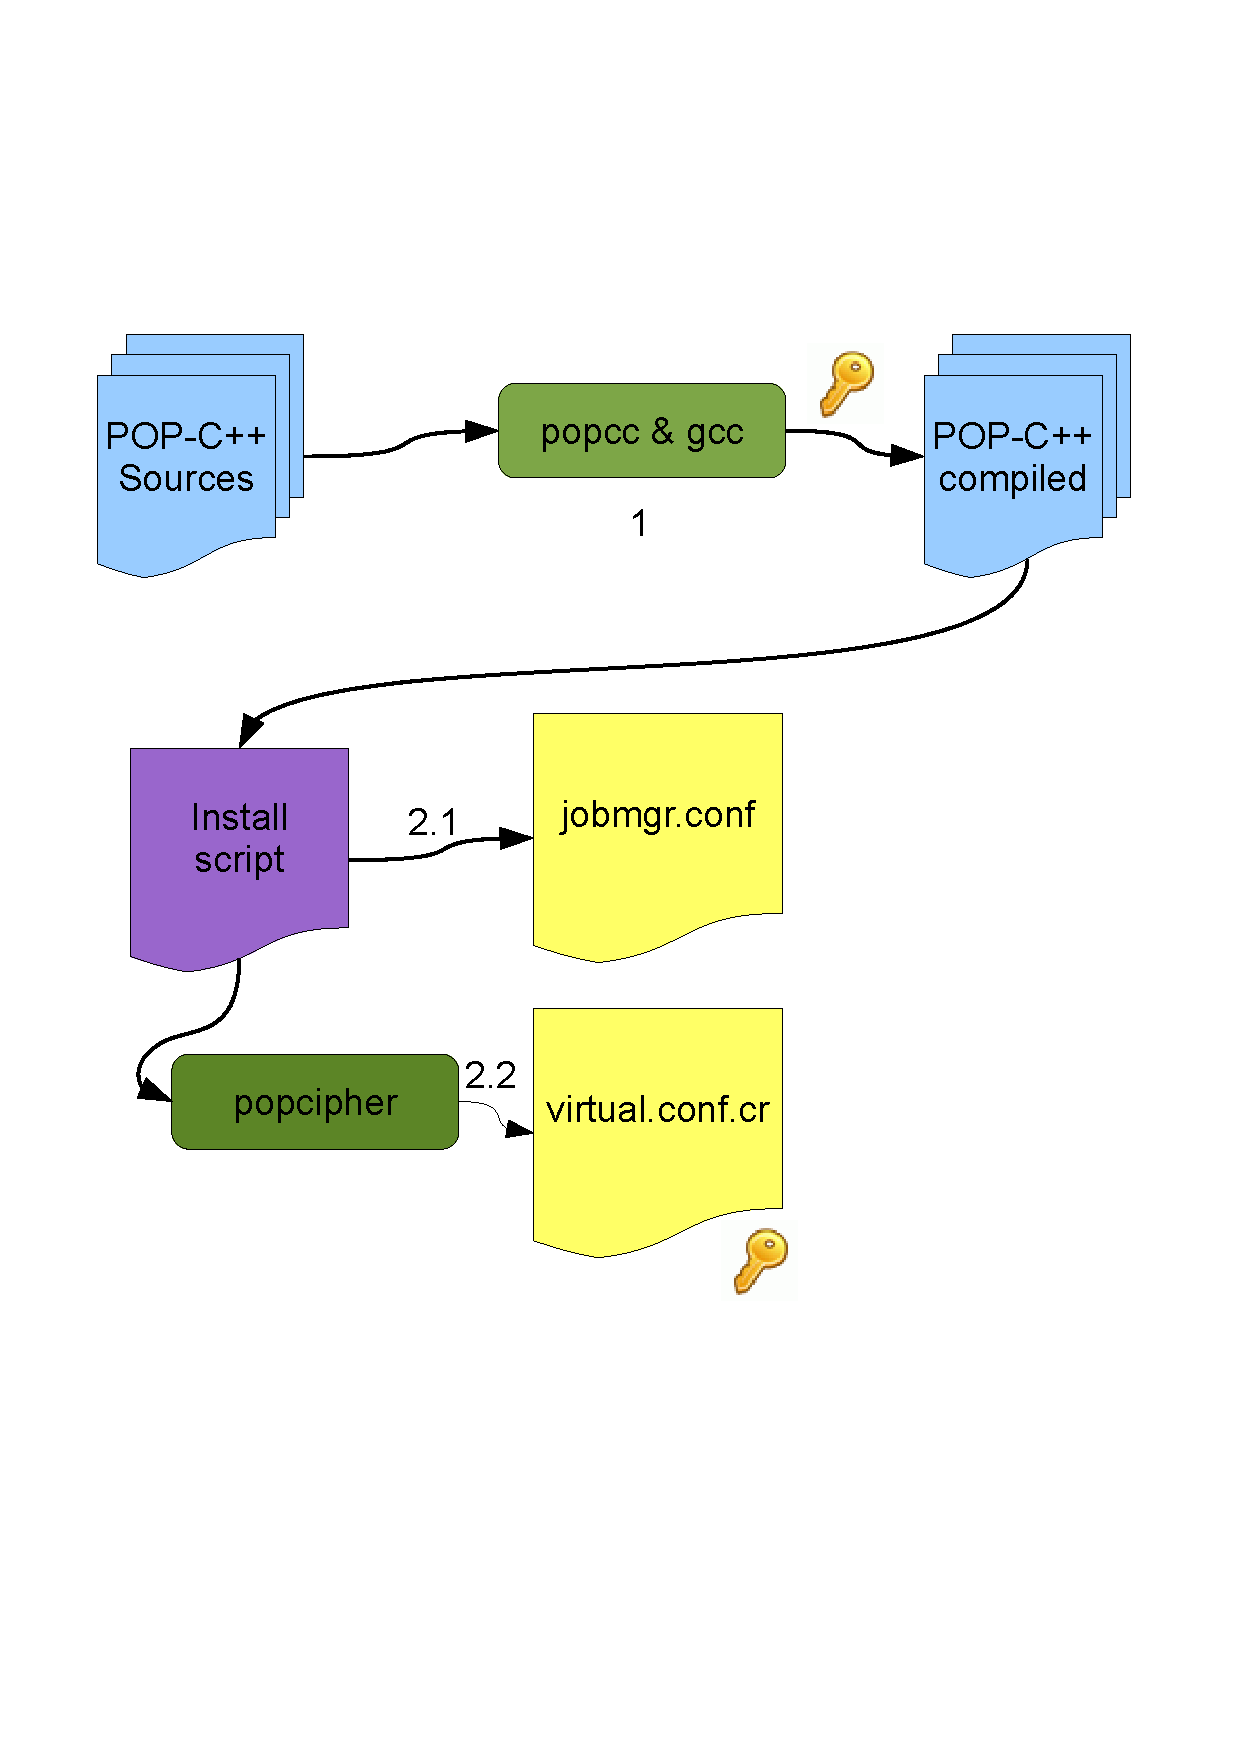
\includegraphics[width=0.5\textwidth]{./pic/cipher1.pdf}
	\label{fig:cipher1}
\end{figure}


Once the virtual configuration file is encrypted, POP-C++ need a way to read these information. Figure \ref{fig:cipher2} shows the starts of the POP-C++ Global Services. Once the Virtual Secure JobMgr (VirtSecureJobMgr) is stared by the "SXXpopc" script, this object will read the virtual.conf.ci file. This object has the ability to decipher this file as during the compilation of POP-C+, the generated key has been included in its executable. The VirtSecureJobMgr decipher the virtual.conf.ci file and use its information directly in memory. All the information located in the jobmgr.conf file are read as usual as they are all in clear. \s
\begin{figure}[ht]
	\caption{POP-C++ Virtual Configuration - Cipher - Step 2}
  	\centering
	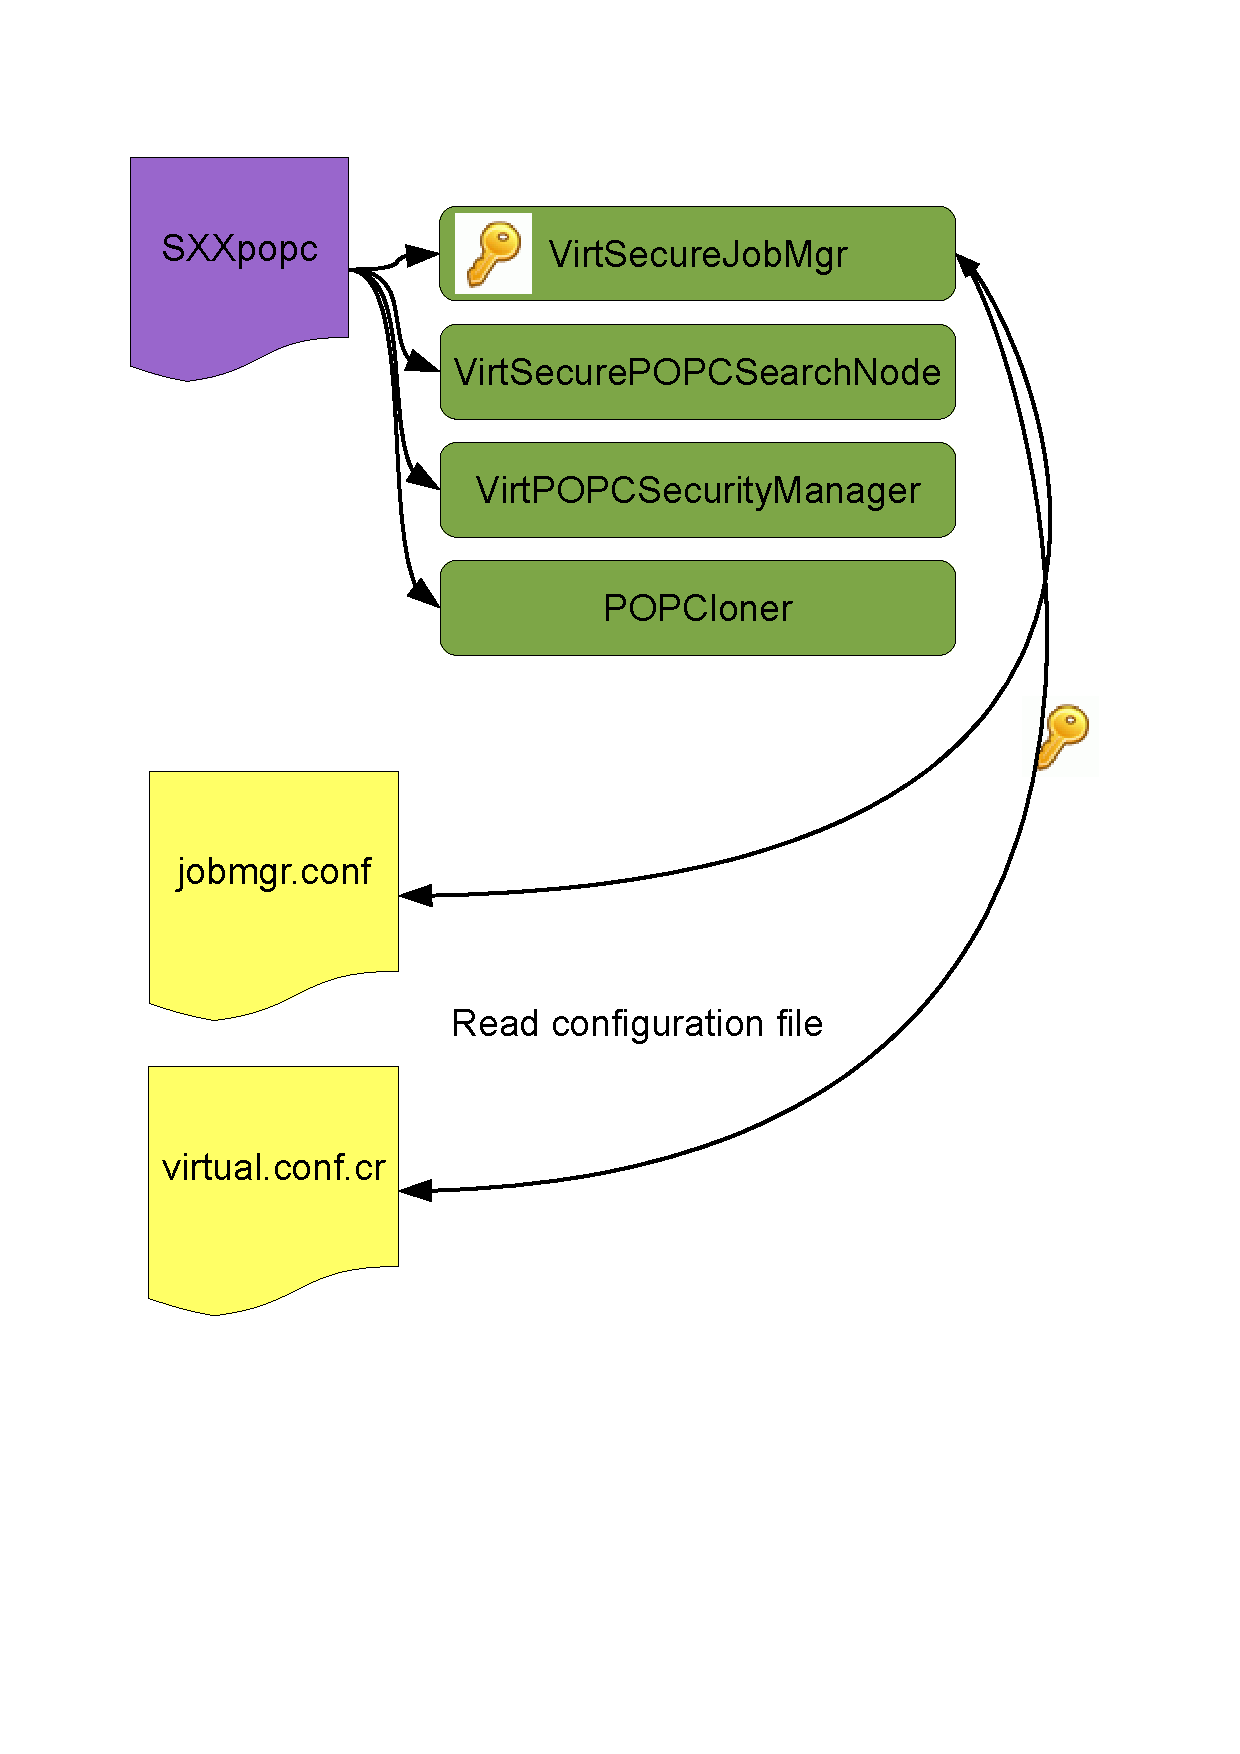
\includegraphics[width=0.5\textwidth]{./pic/cipher2.pdf}
	\label{fig:cipher2}
\end{figure}


\pagebreak
%
% POP APPLICATION IDENTIFIER
%
\subsection{POP Application Identifier}
The AppCoreService has been modified to generate the POP Application ID. This ID is generated in the constructor of this object. The "Request" object has also been modified to include this ID. Just before launching the resource discovery, the JobMgr will contact the AppCoreService to know the POPAppID and set it in the request. The other JobMgrs contacted will know for which application a request has been launched. \s

For more information about the POP Application Identifier, please refer to the document "POP-C++ over SSH Tunnel"\cite{popcssh} in section 7.1.\s

In addition to these modifications, the reservation process must also include the POPAppID and the RequestID. The "struct Resources" defined in \textbf{./lib/jobmgr.ph} have been modified to include the POPAppID and the RequestID. The "Reserve" method must now accept the POPAppId and the RequestID as parameters. At this point, the JobMgr has all the information to manage the different Worker VM.\s

\textbf{Files modified : } ./include/request.h, ./include/Makefile.am, ./lib/request.cc, ./lib/appservice.ph, ./lib/appservice.cc, ./lib/jobmgr.cc, ./lib/Makefile.am\s

\textbf{Files added : } ./include/popwayback.h, ./lib/popwayback.cc



\subsection{Modification of the VPopCWrapper}
\label{lb:wrapper}
The VPopCWrapper was designed to use only one worker VM at the same time. To be able to manage more than one worker, the VPopCWrapper has been changed. A POPvm object has been created to encapsulate all the information relative to a Worker VM. This object is then passed to some of the wrapper method. Each POPvm object has a pointer to its own domain (pointer of domain is a notion introduced by libvirt). This pointer is saved and then any operation of the wrapper can be executed on this VM. \s

The POPvm object encapsulates the following information at the moment : \s
\begin{enumerate}
\item The VM name (displayName)
\item The VM configuration file (VMX file on ESXi)
\item The VM volume (datastore on ESXi)
\item The VM OS
\item The VM clean snapshot
\item The VM IP address
\item The POPAppID (if the VM is reserved)
\item The VM PKI 
\item The VM state (free, reserved, busy)
\end{enumerate} 


The VPopCWrapper interface has been changed to use this new object and be more flexible. The new interface looks as follows : 
\begin{itemize}
\item int \_popc\_connectOpenAuth(string uri, string user, string password);
\item int \_popc\_connectClose();
\item virDomainPtr \_popc\_domainLookupByName(string domName);
\item int \_popc\_domainState(POPvm \&vm, string* state);
\item long long \_popc\_nodeGetFreeMemory();
\item int \_popc\_nodeGetinfo(nodeInfo* info);
\item int \_popc\_domainSnapshotNum(POPvm \&vm);
\item int \_popc\_domainSnapshotListNames(POPvm \&vm, string names[], unsigned short len);
\item int \_popc\_domainRevertToSnapshot(POPvm \&vm, string snapshotName);
\item int \_popc\_domainRevertToOldestSnapshot(POPvm \&vm);
\item int \_popc\_domainSnapshotCreate(POPvm \&vm, string name, string description);
\item int \_popc\_domainSnapshotDelete(POPvm \&vm, string snapshotName, bool removeChildren = false);
\item int \_popc\_domainSetMemory(POPvm \&vm, unsigned long memoryInKb);
\item int \_popc\_domainSetMaxMemory(POPvm \&vm, unsigned long memoryInKb);
\item long \_popc\_domainGetMaxMemory(POPvm \&vm);
\item int \_popc\_domainShutdown(POPvm \&vm);
\item int \_popc\_domainSuspend(POPvm \&vm);
\item int \_popc\_domainResume(POPvm \&vm);
\item const string \_popc\_domainGetMac(POPvm \&vm);
\item int \_popc\_domainGetIpAddress(POPvm \&vm);
\item int \_popc\_domainIsConnected(string domName="");
\item int \_popc\_sendLocalPublicKey(POPvm \&vm);
\item int \_popc\_sendPublicKey(POPvm \&vm, POPString pki);
\item int \_popc\_getLocalPublicKey(POPvm \&vm);
\item int \_popc\_domainClone(POPvm \&original, POPString baseName, int suffix, paroc\_accesspoint clonerAP);
\item int \_popc\_domainWaitingForTools(POPvm \&vm);
\item const string \_popc\_getError();
\end{itemize}

In addition to the modifications above, some of the methods in the ESX implementation of the wrapper have been modified to use the VIX API instead of launching shell command. These changes are explained in Section \ref{lb:vix}.\s

A basic implementation of the VPopCWrapper is done in with the object POPWrapper. This object implements all the methods that can be implemented with libvirt. The ESXWrapper extends the POPWrapper and re-implements only the needed methods. Figure \ref{fig:wrapper_cd} shows the class diagram of wrapper objects. 

\begin{figure}[ht]
	\caption{Virtual Wrapper - Class Diagram}
  	\centering
	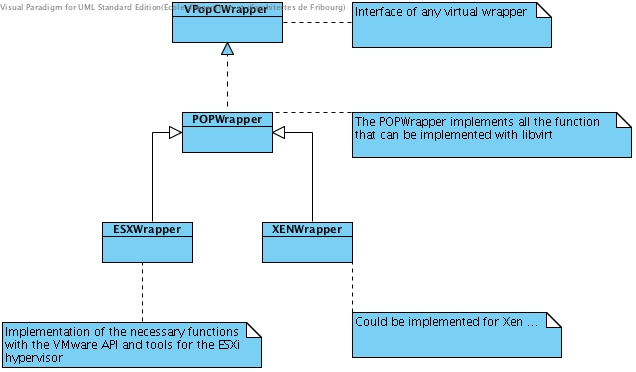
\includegraphics[width=1.0\textwidth]{./pic/wrapper_cd.jpg}
	\label{fig:wrapper_cd}
\end{figure}


%
% VIX COMPILATION
%

\pagebreak
\subsection{POP-C++ and VIX}
\label{lb:vix}
As said in Section \ref{lb:wrapper}, the VIX API is used for some methods in the ESX implementation of the wrapper. These methods were using shell command to do their tasks. It's way better to use API call to perform those actions. Libvirt could one day implement the needed functions available in VIX. If so, the ESX implementation should be modified. 

\subsubsection{Include VIX in the compilation process}

All the necessary modifications done in the configuration script and makefile to include VIX in the compilation process are listed below.\s

\textbf{File: configure.ac:}\\
As the VIX API does not install a ".pc" file for the pkg\_config function. We have to declare the \_CFLAGS and the \_LIBS marcos for VIX. The lines below have been added to the "configure.ac" file. \s

\begin{lstlisting}
VIX_CFLAGS="-lvixAllProducts -ldl"
VIX_LIBS="-I/usr/include/vmware-vix"
AM_SUBST([VIX_CFLAGS])
AM_SUBST([VIX_LIBS])
\end{lstlisting}\s

\textbf{File: ./lib/Makefile.am:}\\
The input Makefile located in the "lib" directory must also be modified. The VIX macros must be added to the macro "AM\_CXXFLAGS". \s

\begin{lstlisting}
AM_CXXFLAGS= OTHER_FLAGS $(VIX_CFLAGS) $(VIX_LIBS)
\end{lstlisting}\s

With those modifications, POP-C++ can now be compiled with the VMware VIX API. \s

\textit{NOTE:} The VIX API must be installed on the machine which compile POP-C++ in its Virtual or Virtual-Secure version. 


\subsubsection{Using VIX to get the worker VM IP address}
The VIX API allow us to read some properties on the guest VM. This ability is used to read the IP address of the guest VM. The process is going as follows:

\begin{enumerate}
\item Connect to the hypervisor (VixHost\_Connect())
\item Get a pointer to the VM (VixHost\_OpenVM())
\item Power on the VM if not running (VixVM\_PowerOn())
\item Waiting for the VMware tools to be ready (VixVM\_WaitForToolsInGuest())
\item Read the variable "ip" (VixVM\_ReadVariable())
\end{enumerate}\s

\textit{NOTE:} For the full code, please see the file ./lib/ESXWrapper.cc method "\_popc\_domainGetIpAddress(POPvm \&vm);"

\subsubsection{Using VIX to send and write the admin VM public key on worker VM}
The VIX API has two very interesting functions that allow us to send a file on the worker VM and to execute a command on the worker VM. To transfer the Admin VM PKI to the Worker VM, we can send the public key file and write it in the authorized\_keys file on the Worker VM by executing a shell command. The process to do this using VIX is going as follows: \s

\begin{enumerate}
\item Connect to the hypervisor (VixHost\_Connect())
\item Get a pointer to the VM (VixHost\_OpenVM())
\item Power on the VM if not running (VixVM\_PowerOn())
\item Waiting for the VMware tools to be ready (VixVM\_WaitForToolsInGuest())
\item Login in the guest VM (VixVM\_LoginInGuest())
\item Copy the Admin VM public key file to the guest VM (VixVM\_CopyFileFromHostToGuest())
\item Execute a command on the guest to write the key (VixVM\_RunProgramInGuest())
\end{enumerate}\s

\textit{NOTE:} For the full code, please see the file ./lib/ESXWrapper.cc method "\_popc\_sendLocalPublicKey(POPvm \&vm);"

\subsubsection{Using VIX to execute a ping on the Worker VM}
As the Worker VM is reverted from a snapshot, its saved IP address could be used by another computer when reverted. To be sure to have a valid IP address before executing jobs on the Worker VM, the guest will ping the Admin VM. This procedure will change the guest IP address if this one is invalid on the network. To execute this action, the wrapper uses the VIX API as well. The process is going as follows: 

\begin{enumerate}
\item Connect to the hypervisor (VixHost\_Connect())
\item Get a pointer to the VM (VixHost\_OpenVM())
\item Power on the VM if not running (VixVM\_PowerOn())
\item Waiting for the VMware tools to be ready (VixVM\_WaitForToolsInGuest())
\item Login in the guest VM (VixVM\_LoginInGuest())
\item Execute a ping on the guest to contact the Admin VM (VixVM\_RunProgramInGuest())
\end{enumerate}\s

\textit{NOTE:} For the full code, please see the file ./lib/ESXWrapper.cc method "\_popc\_reversePing(POPvm \&vm, POPString ipAdress);"


\pagebreak
\subsection{Cloning function implementation}
As no built-in cloning function is currently implemented either in the VIX API or in libvirt, this function has been implemented from scratch. Cloning a VM takes quite some time. Due to that, a parallel object will be in charge of the whole process and let the others Global Services do their respective tasks. The POPCloner object is launched at the Global Services start up in the Virtual and Virtual-Secure version. This object is initialized with the ESXi hypervisor information.\s

When the Admin VM needs to launch a cloning process, a free Worker VM will be reserved as the original VM. This original VM can be used to clone more than one VM. The Admin VM will do a call to the POPCloner and gives the information relative to the orginal VM. The original VM will be busy during the whole process. Once the cloning process is done, the new VM will be added to the list of managed VM and the original VM will be freed. Unfortunately, the cloning process needs several proprietary tools from VMware. Here is the list of those tools : \s

\begin{itemize}
\item VMware VIX API 1.10.2 or later
\item VMware CLI 4.1 or later
\item VMware tools 8.3.2 or later
\end{itemize}\s


The cloning process is detailed below and each action associated with the needed tool/command.

\begin{enumerate}
\item Create a new POPvm object with the information of the new VM.
\item Check if the original is suspended or running and shut it down if it's the case. The original VM \textbf{must} be shutdown to perform the cloning actions (VIX).
\item Retrieve the configuration file (.vmx) of the original VM (vmware-cmd).
\item Create the new folder for the cloned VM (vifs).
\item List all the files in the original folder and filter them (vifs).
\item Copying files from the original to the new created folder (vmkfstools and vifs).
\subitem The .vmx file is read and a new one is created for the new VM.
\item Register the cloned VM (vmware-cmd).
\item Remove useless temporary files
\item Write the VM information in the Virtual JobMgr configuration file. 
\item Start and stop the cloned VM (VIX). This step is fundamental to be able to retrieve the VM with libvirt. 
\item Add the new VM in the list of usable VM (POP-C++ call to the JobMgr).
\end{enumerate}

\textit{NOTE:} For the full code, please see the file ./lib/popcloner.cc.

\textbf{On going development}\\
Even this function is fully functional, we are currently trying to implement this process directly into the libvirt library. As it is still under development, no information can be given now. 

%\subsection{Requirements}
%To be able to run the POP-C++ Virtual version, the following requirements must be fulfilled:

%\begin{center}
%\begin{tabular}{|p{1.8cm}|p{3.3cm}|p{2.7cm}|p{2.6cm}|p{1.5cm}|p{1.5cm}|}
%\hline
%\textbf{VM Type} & \textbf{POP-C++ version}	& \textbf{VMware tools} & \textbf{VMware CLI} & \textbf{VIX} & \textbf{libvirt}\\ \hline
%Admin & Virtual Secure & X & >= 4.1 & >= 10.1 & >= 0.8.5\\ \hline
%Worker & Secure & X & - & - &- \\ \hline
%\end{tabular}
%\end{center}\s

%\begin{itemize}


%\item VMware ESXi 4.1 or later must be installed as the hypervisor.
%\item The VMware tools 8.3.2 build-257589 or later must be installed on the worker VM and on the Admin VM.
%\item The VIX API 1.10 or later must be installed on the admin VM.
%\item libvirt 0.8.3 or later must be installed on the admin VM.
%\end{itemize} 


\pagebreak
\subsection{Reservation process}
The original reservation process of POP-C++ does not take into consideration the VM. To be able to reserve a VM for a specific POP-C++ Application (POPAppID), the "Reserve()" method has been reimplemented for the Virtual and Virtual-Secure JobMgr. Figure \ref{fig:flowchart_reservation} shows a flowchart of the reservation process for both Virtual and Virtual-Secure version. \s

\begin{figure}[ht]
	\caption{Reservation process}
  	\centering
	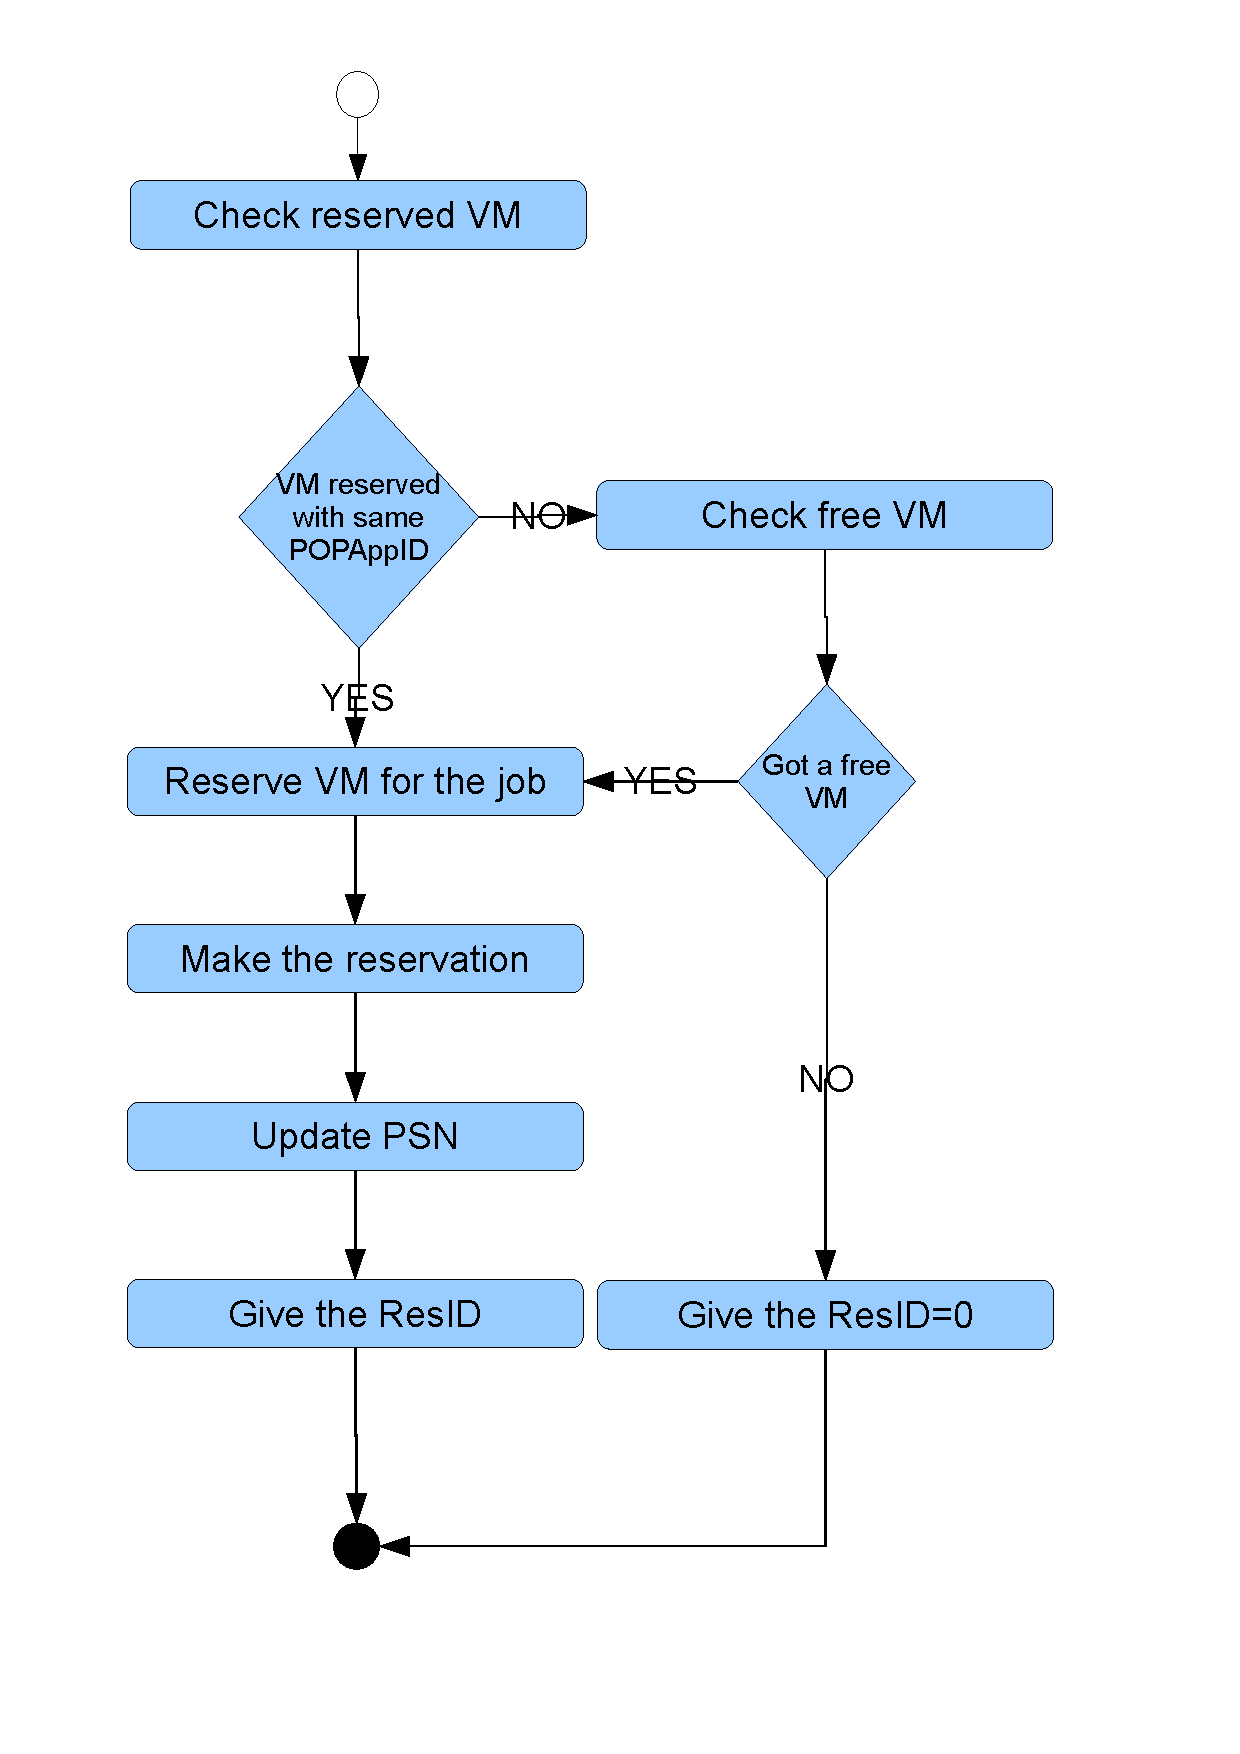
\includegraphics[scale=0.5]{./pic/reserve_vm.pdf}
	\label{fig:flowchart_reservation}
\end{figure}

\pagebreak
\subsection{Preparing a VM to execute a Job}
As POP-C++ is now Virtual and Secure, the preparation of the VM to execute a job is a little bit different. Figure \ref{fig:flowchart_preparation} shows the flowchart of the VM preparation before the job execution.

\begin{figure}[ht]
	\caption{VM Preparation}
  	\centering
	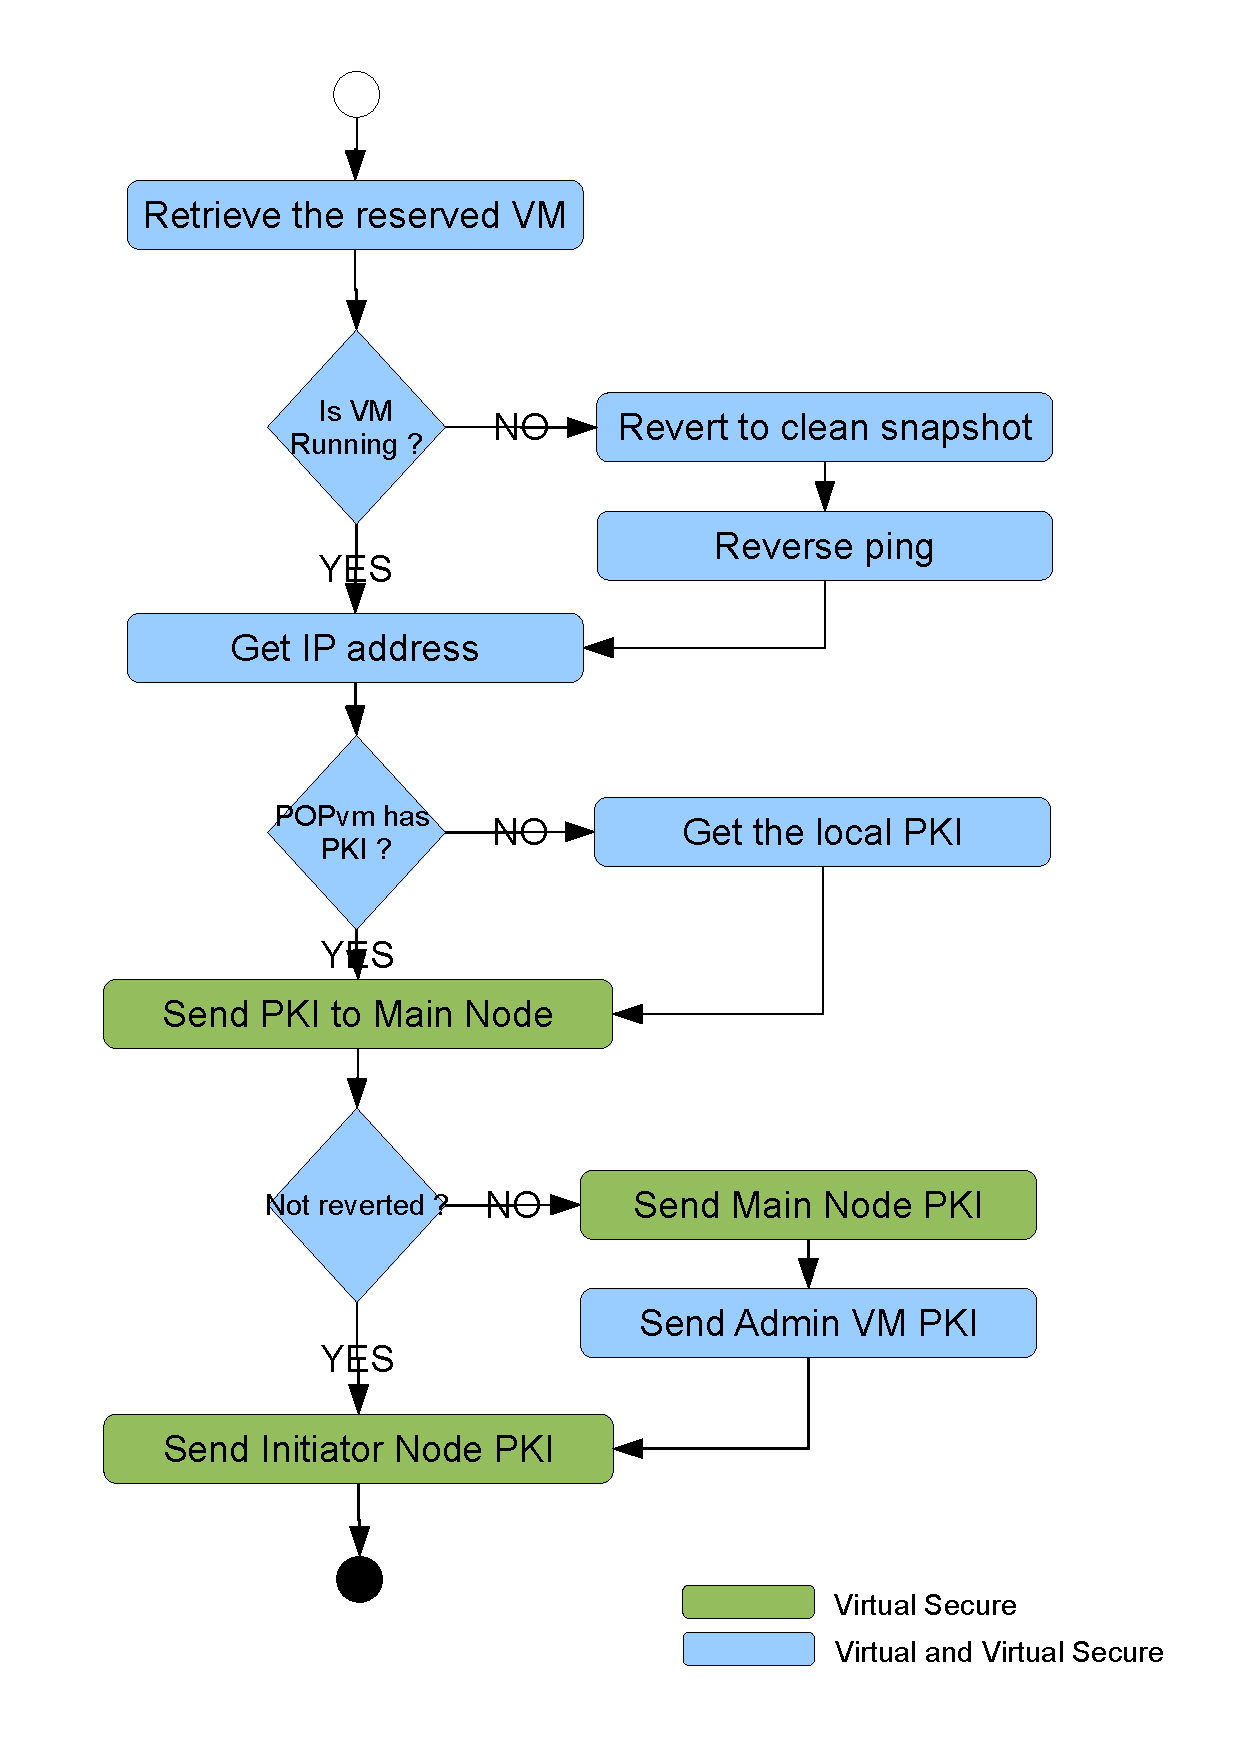
\includegraphics[scale=0.5]{./pic/prepare_vm.pdf}
	\label{fig:flowchart_preparation}
\end{figure}

\pagebreak
\subsection{How to know the Global Services that start an object}
A Worker VM do not have Global Services running on it. When an object is created from another object located on the Worker VM, the interface of this worker needs to know which Global Services has created its broker. This information is fundamental to use the key routing process implemented in the POP-C++ Security Manager as the creator node is the node that will write and send the PKIs. This information is known by the JobMgr just after the resource discovery. To be able to give this information back to the Interface, the method "CreateObject()" of the JobCoreService has been changed a little bit. Here is the new signature of this method. \s

\begin{lstlisting}
sync conc virtual int CreateObject(paroc_accesspoint &localservice, const 
paroc_string &objname, const paroc_od &od, int howmany, [in, out, 
size=howmany] paroc_accesspoint* jobcontacts, int howmany2, [in, out, 
size=howmany2] paroc_accesspoint* remotejobcontacts);
\end{lstlisting}\s

The array "remotejobcontacts" will hold the JobMgr access point that created the object as the array "jobcontacts" hold the access point to the object itself. \s

\textit{NOTE:} The parameter "howmany2" is not mandatory in pure POP-C++ as "howmany" could be used for the second array size. This parameter has been added to keep the compatibility with POP-Java. 


\subsection{Virtual POP-C++ Security Manager}
The POP-C++ Security Manager (PSM) developed in "POP-C++ over SSH Tunnel" is not able to manage a "virtual node" with an Admin VM and some Worker VM. To manage the security of the virtual node, the Virtual POP-C++ Security Manager has been developed. This parallel object inherits from the orginal PSM. \s

In POP-C++ VS, the VirtualPOPCSecurityManager (VPSM) works as a router for the PKI. This parallel object will receive request from others nodes in the GRID but also from the Worker VM associated on its own node. With the POPAppID, the VPSM is able to operate a kind of key routing. This chapter explains the modifications done for this routing process. 

\subsubsection{Add new mapping for Request PKI}
When the Admin VM sends a resource discovery request, all the possible resources will answer with their respective PKI. Unfortunately, the VM that will execute this job is maybe not defined yet. To be able to send the PKI of the chosen resource the the VM, a new mapping has been added in the Virtual PSM. This mapping maps a combination of the POPAppID and the ReqID with the PKI. \s

When a node receives a resource discovery request, it saves the PKI in the mapping. If this node is asked to execute the job, the PKI will be retrieved and sent to the VM.\s

\textbf{Files modified: } ./lib/virtual\_popc\_security\_manager.ph, ./lib/virtual\_popc\_security\_manager.cc, ./lib/virtual\_secure\_popc\_search\_node.cc

\subsubsection{Write the key on a VM}
When a key reaches the PSM, this key must be written on the right VM. As each running Worker VM is attached with a POPAppID, it's easy to find the right VM to write a key if we know the POPAppID associated with this key. \s

Once the VM is retrieved, the VPopCWrapper method "\_popc\_sendPublicKey(POPvm \&vm, POPString pki);" is used to write the key on the Worker VM.\s

\textbf{Files modified:} ./include/VPopCWrapper.h, ./include/ESXWrapper.h, ./lib/ESXWrapper.cc, ./lib/virtual\_popc\_security\_manager.ph, ./lib/virtual\_popc\_security\_manager.cc


\subsection{Application ending}
The POP-C++ runtime must handle the end of a POP-C++ application. The application services destruction can inform the of the end of a POP-C++ application. Once the destructor of the AppCoreService will be called, a call will be propagated to the JobMgr's method "ApplicationEnd(POPString popAppId, bool initiator)". This method will just remove the associated reservation in the standard version. In the Virtual and Virtual-Secure version, this method will suspend any VM reserved for this POPAppID. \s

\textbf{Files modified:} ./lib/appservice.cc, ./lib/jobmgr.ph, ./lib/jobmgr.cc, ./lib/virtual\_jobmgr.ph, ./lib/virtual\_jobmgr.cc


\subsection{Unique starting Worker VM}
As we are able to clone VM, the assumption of a unique worker VM at first start-up is made. On the first start-up, depending on the configuration entered by the user during the installation, some VM can be cloned. This new VM will not appear in the virtual configuration file as we can find them at global services start-up. \s

To be able to do this task, the first VM must respect an important rule. The name of the first worker VM must finish with \textbf{\_worker1}.


\subsection{Using valgrind to detect memory leaks}
Valgrind is a set of tools to detect incorrect memory management in a program. We try to run the POP-C++ Global Services through valgrind to remove any possible leaks or incorrect memory management. \s

\textbf{Running the Interface-side with valgrind}\\
As POP-C++ program are divided into several parts, each part must be run with valgrind. For the Interface-side, the "popcrun" script must be modified to included the valgrind command and options. Here are the modifications made to run the Interface-side with valgrind : \s

\begin{lstlisting}
cmd="valgrind --log-file=/tmp/$PROG$$ $PROG $args -initparoc 
-appservicecode=${MYAPPSERVICE} ${MY_PROXY} -codeconf=${PATHCONF}
/${FILECONF} -jobservice=${MYJOBSERVICE} ${localFlag}"
\end{lstlisting}\s

Some leaks have been detected by using valgrind but not all of them are currently corrected. 
\textbf{----- TODO TODO TODO -----} \textit{finish valgrind and wrote conclusion}

\textbf{Running the Broker-side with valgrind}\\
To run the Broker side with valgrind, we need to change the 

\textbf{---- TODO ----}
\s

%####################################
%
% GENERAL MODIFICATION ON POP-C++
%
%####################################
\pagebreak
\section{General modifications}
\label{sec:gen_mod}
This chapter regroups all the modifications made on POP-C++ in general. Some of these modifications have been made to fix bugs and some to enhance to possibilities of POP-C++ in all versions. 

\subsection{Update the POP-C++ Search Node resource information}
Currently, the POP-C++ Search Node (PSN) is not updated when a reservation is made on the node. To fix this bug, the PSN has now two additional methods to add a job and to remove a job. With this update, the PSN can directly refuse a resource discovery and not send a response and refuse the reservation later.\s

These methods increase or decrease the resources of the PSN and the number of job currently executed on the node. Here are the signature of these two methods : \s
\begin{lstlisting}
sync seq void addJob(float power, float memorySize, float bandwidth);
sync seq void removeJob(float power, float memorySize, float bandwidth, 
     int nbJob);
\end{lstlisting}

To reduce the number of call to the PSN, the removing method is called once for all the application. 


% Securty assumptions
\pagebreak
\section{Security assumptions}
\label{sec:security}
This chapter aims to explain what we think are strengths and weaknesses on a security point of view in this project. The first section will focus on the strength as the second one will focus on the weaknesses. \s

\subsection{Security strengths}

\subsubsection{Application isolation}
An application is isolated from other application as a Worker Vm is started for each different application on a node. This means that an application can only disturb itself but not other running application.

\subsubsection{Admin VM isolation}
The Admin VM is totally isolated from the execution of the POP-C++ application. This VM do not accept other public key than the ones exchanged for the confidence link. An application should never be launched from an Admin VM. 

\subsubsection{Worker VM clean state}
A Worker VM is always reverted to its clean state before executing an application. Of course, this clean state depends on the person who created it during the installation of the node. 


\subsection{Security weaknesses}
\subsubsection{Node running the main}
Every POP-C++ application has a start point which is the main. The main must run on a node we will called the Main Node. The Main Node could be vulnerable has it will accept several public key from the worker used for this application. For the moment, we did not develop a perfect solution for this problem but some ideas are drawn in Section \ref{sec:future}.

\subsection{Possible security attacks}
This section aims to expose some of the possible attacks we found possible to happen on our middle-ware and the way to avoid them. 

\subsubsection{Sniffing the network}
By sniffing the network, the possible hacker could not do anything to our confidence network. Every connections are encrypted into a SSH Tunnel. 

\subsubsection{Hacking the Admin - VM}
An external person could hack into the Admin VM. As the Admin VM just acts as a routing point for the key exchnage, 

\subsubsection{Enter the confidence network with a fake POP-C++}
A malicious developer could modify POP-C++ before installing it. This means that a different version of POP-C++ will enter a confidence network with standard POP-C++ VS. This kind of hack could disturb the good working of an execution. As the key transferred between the node are the public key, they do not pose a security issues if they are intercepted. 

\subsubsection{Make a POP Application with back doors}
A developer could make a POP Application that keep some process alive after its execution. As only one application is running in a Worker VM and these Worker VM are reverted at end, this kind of hack pose no problem to our middle-ware.



% Functionality and performance tests
\pagebreak
\section{Test}
\label{sec:test}
This chapter explains all the tests done on the new version of POP-C++ to be sure that this version is functional. The second part of this chapter is a report on the performance of the new version.


% ############################
%
% ----- BASIC FUNCTIONAL TESTS ---
%
% ############################
\subsection{Functional tests}
With the key exchange process, some functional tests have been made to verify the correct behaviour of this key exchange. This test are the same as the ones explained in the "User Manual" add-on.



% ############################
%
% ----- REAL SITUATION TESTS -----
%
% ############################
\subsubsection{Real situation test}
To prove our theory, a real test situation has been put in place at EIA-FR. This section will explain the infrastructure and the constraints of this situation. \s

\textbf{\textit{TODO}}: if test with Geneva done, include all the details. \s

\textbf{EIA-FR test infrastructure}\\
The GRID \& Cloud Computing Group has got a DMZ that can be managed without the intervention of the IT Head Office of the school. This DMZ is delimited from the Internet by a firewall (FW). This FW is able to manage different areas. These areas are working as different networks. Nowadays, four different areas are in place. 

\begin{itemize}
\item "Grille Collaborateurs" - Collaborators GRID
\item "Grille étudiants" - Students GRID
\item "Servers"
\item "Grille Test" - Test GRID
\end{itemize}

Figure \ref{fig:eia_dmz} shows the current configuration of the EIA-FR DMZ

\begin{figure}[ht]
	\caption{EIA-FR DMZ}
  	\centering
	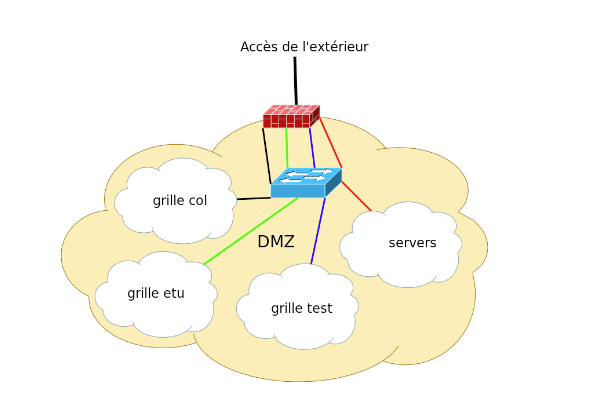
\includegraphics[scale=0.6]{./pic/dmz1.png}
	\label{fig:eia_dmz}
\end{figure}

The subnet 160.98.22.0/23 is available for the computers located in the DMZ. \s

\textbf{Restriction}\\
The only restriction imposed by the IT Head Office is to block the SMPT port (25) and the SMPT-S port (587). This restriction avoid the unwanted use of a mail server installed in the DMZ as a routing server for SPAM. This problem could put the all school network (160.98.0.0) to be on a blacklist. \s

\textbf{Area}\\
The IP address range 160.98.22.1 to 160.98.22.254 is subdivided as follows:

\begin{center}
\begin{tabular}{|p{2.5cm}|p{2.5cm}|p{2.5cm}|p{2.5cm}|}
\hline
\textbf{Area} & \textbf{Subnet}	& \textbf{Gateway} & \textbf{Mask}\\ \hline
Grille étudiants & 160.98.22.0 & 160.98.22.1 & 255.55.255.192 \\ \hline
Grille collaborteurs & 160.98.22.64 & 160.98.22.65 & 255.55.255.192 \\ \hline
Grille test & 160.98.22.128 & 160.98.22.129 & 255.55.255.192 \\ \hline
Servers & 160.98.22.192 & 160.98.22.193 & 255.55.255.192 \\ \hline
\end{tabular}
\end{center}\s

Rules have been globally defined for each area. Some specific rules are defined for well defined computers. 

\textbf{Proposition for the ViSaG project}\\
To avoid external access to the internal school network, the school network is simulated by an area in the DMZ. \s

A computer named "Master1", in the rest of this section, will be installed in the area "Grille collaborateur". In the ViSaG project, this computer will be the only access point for HEPIA and HE-Arc. \s

A second computer named "Master2" will be installed in the area "Grille Test". This computer will be accessible by Master1. Master1 and Master2 are physical computer running VMware ESXi.\s

On these computers, a virtual machine (VM) named "Admin" will run permanently. The "Admin" VM on Master1 and the one on Master2 will be able to communicate together because they made the confidence link.
When a request is coming on one "Admin" VM, a "Worker" VM is launched. The computation work will be done in these "Worker" VMs.\s

\pagebreak
A DHCP server need to be set to give IP Address to the "Worker" VM. As shown on Figure \ref{fig:dmz_dhcp1}, the DHCP server will be installed on an "Admin" VM. The IP address distributed by the DHCP server must be public address.

\begin{figure}[ht]
	\caption{DHCP server on "Admin"}
  	\centering
	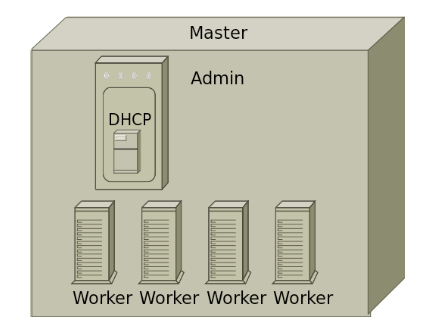
\includegraphics[scale=0.6]{./pic/dmz2.png}
	\label{fig:dmz_dhcp1}
\end{figure}

The DHCP server could also be set on an external VM as shown on Figure \ref{fig:dmz_dhcp2}.

\begin{figure}[ht]
	\caption{DHCP server on an external VM}
  	\centering
	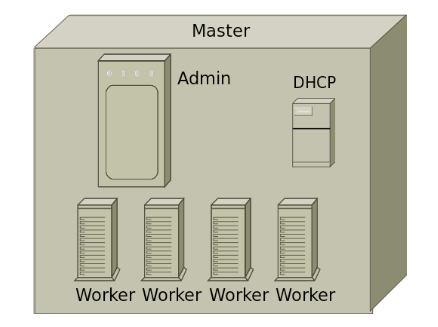
\includegraphics[scale=0.6]{./pic/dmz3.png}
	\label{fig:dmz_dhcp2}
\end{figure}

\textbf{Important point}\\
It is important than only one DHCP server is accessible in an area. The FW will be configured to communicate with a specific computer with a specific IP address. If the "Worker" get his IP address from another DHCP server, this address will be blocked by the FW.\s

In order that the "Worker" managed by the "Admin" on Master1 can communicate with the "Worker" managed by the "Admin" on Master2, the port 22 (SSH) must be open for the IP address attibuted to the "Worker". A number of rules egal to the number of "Worker" + 2 ("Master" + "Admin") must be defined on the FW. To avoid to many rules on the FW, the DHCP server will be configured to attribute only the good number of IP address for the "Worker" VM. \s

\begin{figure}[ht]
	\caption{Logical View of the infrastructure}
  	\centering
	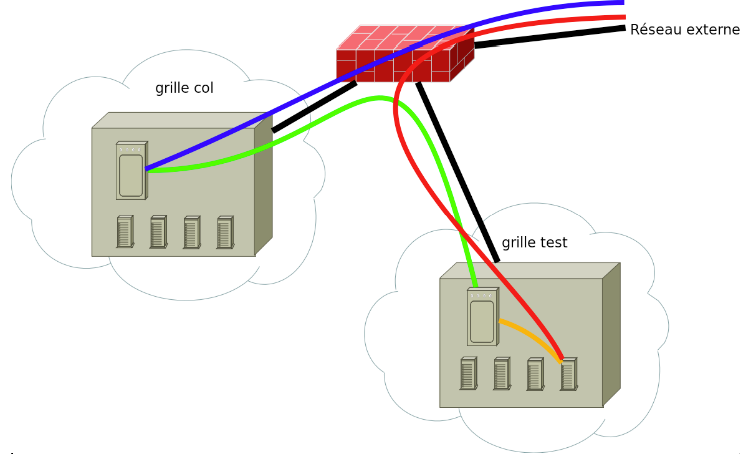
\includegraphics[scale=0.6]{./pic/dmz4.png}
	\label{fig:logical_dmz}
\end{figure}

Figure \ref{fig:logical_dmz} shows a logical view of the DMZ with our two different area working as two different network separated by a FW. The different link color represents: 

\begin{itemize}
\item Black: physical connection
\item Blue: connection on the "Admin" VM
\item Green: Communication between JobMgr
\item Orange: "Worker" creation
\item Red: Communication between "Worker" and the POP-C++ application
\end{itemize}

% ############################
%
% ----- PERFORMANCE TESTS -----
%
% ############################
\subsection{Performance tests}
We were aware that using virtual machine and secure connection will affect the performance of POP-C++. To know which part of the execution is the slowest compared to the standard version, some performance tests have been made. This section explains the different test case and the results.

\subsubsection{Matrix Computation with POP-C++ Standard Version}
To have a basis, we first made performance test on the same architecture but with the Standard version of POP-C++. This section reports all the measures and the results. \s

\textbf{Infrastructure}\\
The infrastructure is composed by three Virtual Machines running on three different ESXi platforms. Each VM have a standard version of POP-C++ installed. The configuration of the global services is made to share the charge between the three nodes. \s

\textbf{Measurements}\\
As the infrastructure for the POP-C++ VS is small, the test for the standard basis version must be done on the same small infrastructure of three nodes. The tests have been performed with three different matrix size and for each matrix size, three different numbers of workers.
\begin{center}
\begin{tabular}{|p{3cm}|p{3cm}|p{3cm}|}
\hline
\textbf{Matrix Size} & \textbf{Nb Workers}	& \textbf{Nb workers/VM} \\ \hline
600x600 & 1 & 1\\ \hline
600x600 & 3 & 1\\ \hline
600x600 & 6 & 2\\ \hline
600x600 & 9 & 3\\ \hline
900x900 & 1 & 1\\ \hline
900x900 & 3 & 1\\ \hline
900x900 & 6 & 2\\ \hline
900x900 & 9 & 3\\ \hline
1200x1200 & 1 & 1\\ \hline
1200x1200 & 3 & 1\\ \hline
1200x1200 & 6 & 2\\ \hline
1200x1200 & 9 & 3\\ \hline
\end{tabular}
\end{center}\s


\subsubsection{Matrix Computation with POP-C++ standard version}
To have a basis for the performance tests on POP-C++ VS, we have run the same tests on the same architecture but with the POP-C++ standard version. This section details the result of these executions. \s

\textbf{Speedup}\\
The speedup has been computed with the different result obtained 
\begin{center}
\begin{tabular}{|p{6cm}|p{2cm}|p{2cm}|p{2cm}|p{2cm}|}
\hline
\textbf{Matrix Size/Nb of workers} & \textbf{1}	& \textbf{3} 	& \textbf{6}	& \textbf{10}\\ \hline
\textbf{600x600} &5.17748 & 2.1383 &	2.3859	& 2.7290 \\ \hline
\textbf{900x900} &16.4920&	6.1572&	6.5519	&7.5837\\ \hline
\textbf{1200x1200} &38.5506 & 13.9942	 & 14.5949 & 16.7564\\ \hline

\end{tabular}
\end{center}\s

\begin{figure}[ht]
	\caption{Speedup for POP-C++ Standard execution}
  	\centering
	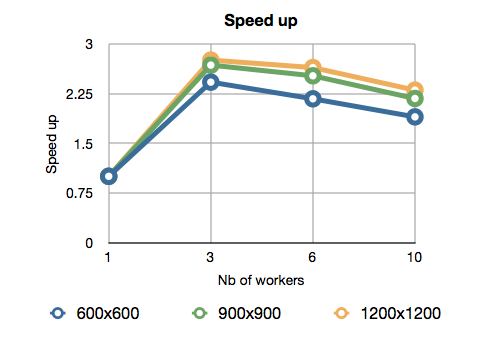
\includegraphics[scale=0.6]{./pic/speedup_std.png}
	\label{fig:speedup1}
\end{figure}

\subsubsection{Matrix Computation with POP-C++ Virtual-Secure version}





% Future development ideas
\pagebreak
\section{Future development}
\label{sec:future}

This chapter will develop several idea that could be implemented in future development of POP-C++ VS. 

\subsection{Pseudo Main Node}
As explained in Chapter \ref{sec:security}, the node running the main of a POP-C++ application is exposed to some risks. To avoid to use the developer node or an Admin VM as the Main Node, a mechanism of pseudo Main Node could be developed. \s

The pseudo Main Node should be a VM running POP-C++ Secure and started by the Admin VM. Figure \ref{fig:pseudomain} shows a schematic view od a ESXi Node running POP-C++ VS and a VM acting as a pseudo Main Node. This mechanism should work as follows:

\begin{enumerate}
\item An application is started on the Admin VM.
\item The Admin VM dected the start of an application, starts the Pseudo Main Node VM and transfer necessary information on this VM. The application is then started from this VM. 
\item The Pseudo Main Node asks for resources to the Admin VM. 
\item The Admin VM starts a worker to give resources to the application.
\end{enumerate}


\begin{figure}[ht]
	\caption{Schematic view of the an ESXi Node with "Pseudo Main Node VM"}
  	\centering
	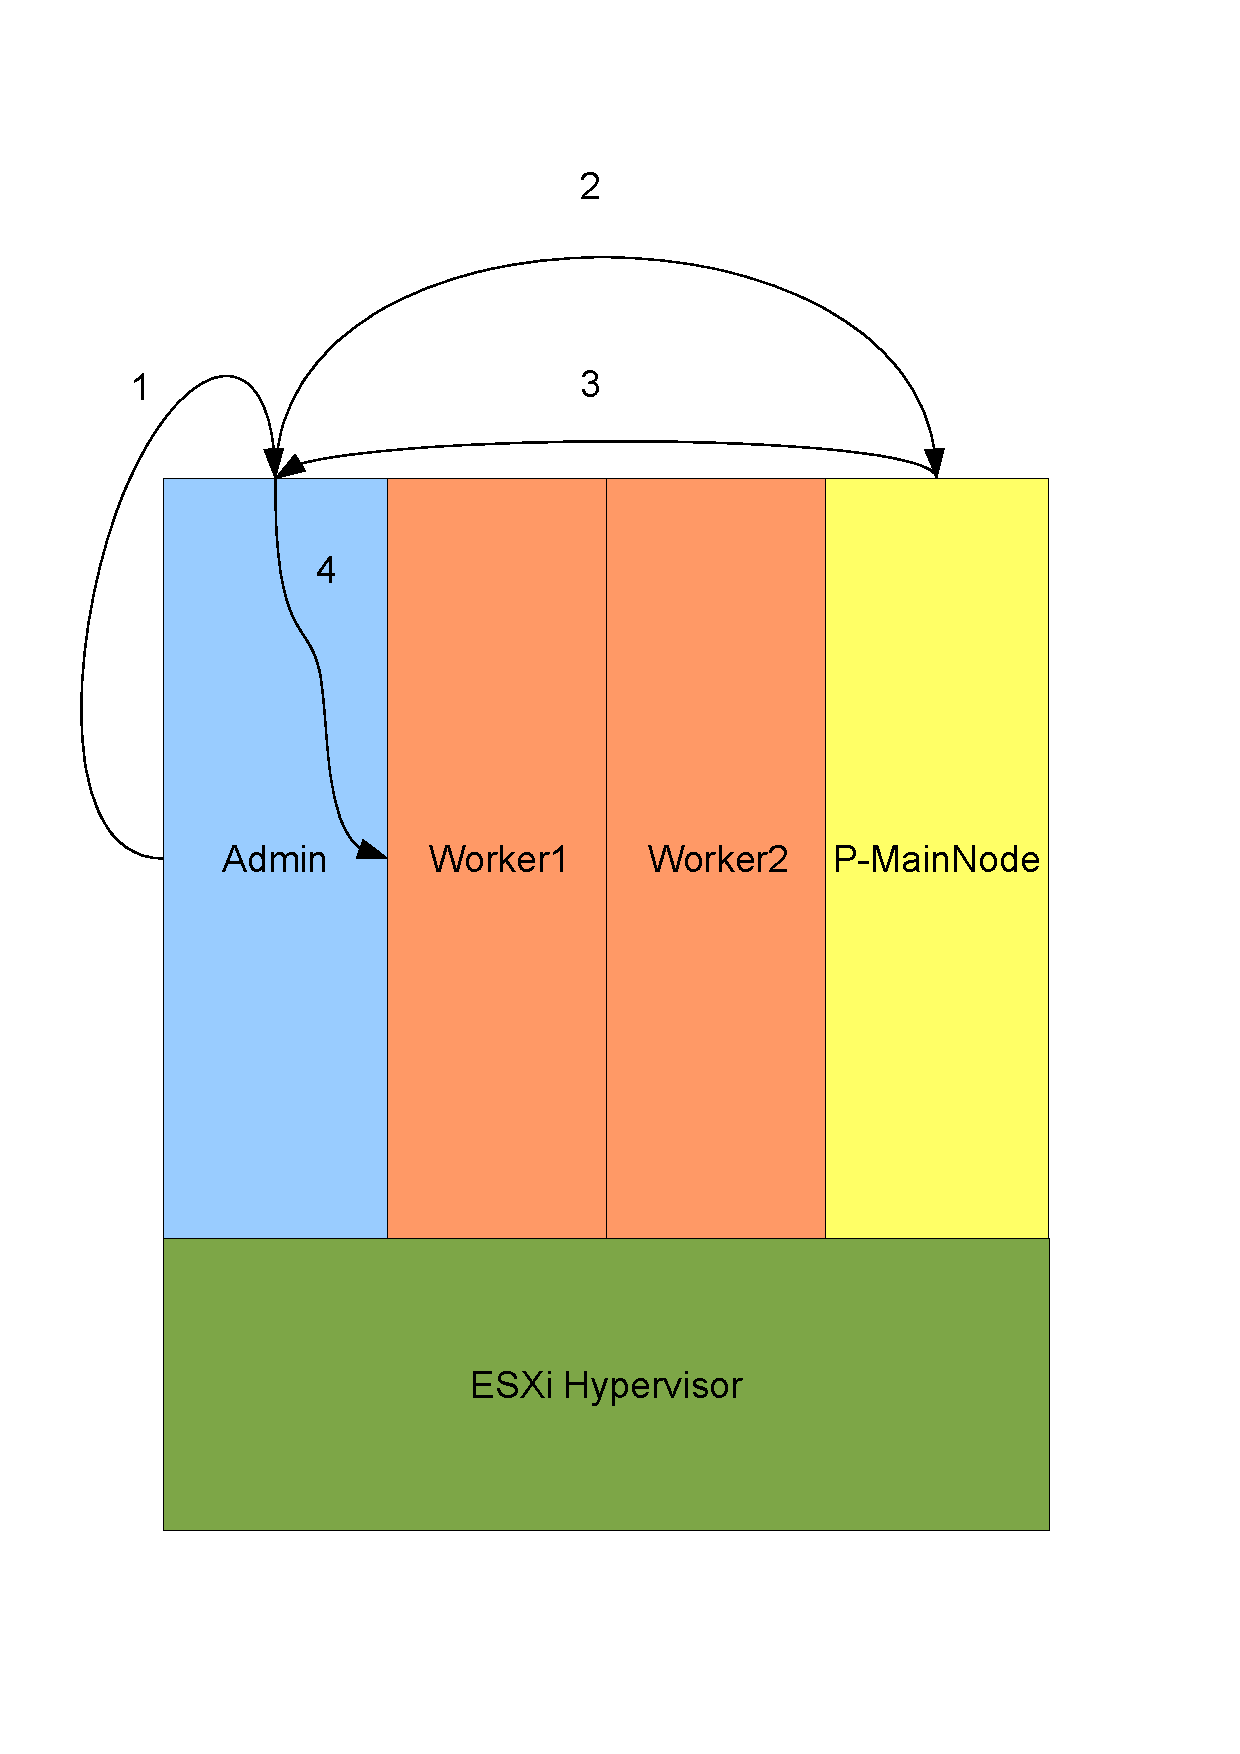
\includegraphics[width=0.5\textwidth]{./pic/pseudomain.pdf}
	\label{fig:pseudomain}
\end{figure}

These steps could be performed by the \textbf{popcrun} script or by the paroc\_main function. 

\subsection{Lock Worker VM}
As Worker VM will execute unknown executable, it could be a great idea to lock as much as possible the outgoing traffic on this VM. On Ubuntu distribution, a simple command line utility named "ufw" allows to apply rules for outgoing and incoming traffic.



\subsection{Keep keys table for each workers}
At the moment, each time a key need to be rerouted, it's done. What could be a great enhancement is to keep a table in the JobMgr about each workers and the keys that have been written on this worker. With this kind of table, we will be able to know if a key has to be wrriten on the worker or not. 

\pagebreak
\section{Glossary}

\begin{itemize}
\item \textbf{API} : Application Programming Interface
\item \textbf{VIX} : API of VMware to interact with the VMware hypervisor (or Workstation ...)
\item \textbf{EIA-FR} : College of Engineering and Architecture of Fribourg
\item \textbf{HEPIA} : Haute Ecole du Paysage, d'Ingénierie et d'Architecte de Genève
\item \textbf{POP-C++ }: Parallel Object Programming C++
\item \textbf{ViSaG} : Virtual Safe GRID
\item \textbf{VM} : Virtual Machine
\end{itemize}


\pagebreak
\section{Table of figures}
\listoffigures{}





%
% REFERENCES
%

\section{References}
\begin{thebibliography}{9}
\bibitem{vpopc1}
	Adrian Wyssen,
  	\emph{VirtualPOPC-1 : Project Report}.
	EIA-FR, Switzerland, 
	June-August 2010.
	
\bibitem{popcssh}
	Valentin Clément,
	\emph{POP-C++ over SSH Tunnel}.
	EIA-FR, Fribourg, Switzerland,
	September-November 2010.
	
\bibitem{popc_vs_addon_manual}
	Valentin Clément,
	\emph{POP-C++ Virtual-Secure : POP-C++ User and Installation manual add-on}.
	EIA-FR, Fribourg, Switzerland, 
	January 2011.

\end{thebibliography}


\end{document}
